% Industrial Attachment Report
% Md. Naimuzzaman -- RUET CSE
% Brain Station 23 -- neoRMS
\documentclass[12pt,a4paper,oneside]{report}

% ===== Packages =====
\usepackage[utf8]{inputenc}
\usepackage[T1]{fontenc}
\usepackage[left=1.25in,right=0.75in,top=1in,bottom=1in]{geometry}
\usepackage{setspace}
\usepackage{graphicx}
\usepackage{float}
\usepackage{booktabs}
\usepackage{longtable}
\usepackage{array}
\usepackage{tabularx}
\usepackage{multirow}
\usepackage{enumitem}
\usepackage{hyperref}
\usepackage{xcolor}
\usepackage{fancyhdr}
\usepackage{titlesec}
\usepackage{tocloft}
\usepackage{listings}
\usepackage{caption}
\usepackage{subcaption}
\usepackage{amsmath}
\usepackage{textcomp}
\usepackage{microtype}
\usepackage{etoolbox}
\appto\sloppy{\hbadness 10000\relax}
\usepackage{tikz}
\usetikzlibrary{positioning,arrows.meta,shapes,shapes.geometric,calc,trees,fit,backgrounds}
\usepackage{pgfplots}
\usepackage[strings]{underscore}
\pgfplotsset{compat=1.18}
\usepackage{qrcode}
\usepackage{xltabular}
\usepackage[most]{tcolorbox}

% ===== Cover page colors =====
\definecolor{corpblue}{RGB}{31,73,125}
\definecolor{primary}{RGB}{31,73,125}
\definecolor{accent}{RGB}{200,120,40}

% ===== Styling =====
\onehalfspacing
\hypersetup{
  colorlinks=true,
  linkcolor=black,
  citecolor=blue,
  urlcolor=blue,
  pdftitle={Industrial Attachment Report -- neoRMS -- Brain Station 23},
  pdfauthor={Md. Naimuzzaman}
}

\graphicspath{{figures/}}

% Code listing style
\definecolor{codebg}{RGB}{248,248,248}
\definecolor{codegray}{RGB}{100,100,100}
\lstdefinestyle{tsstyle}{
  backgroundcolor=\color{codebg},
  basicstyle=\ttfamily\footnotesize,
  breaklines=true,
  frame=single,
  framerule=0.3pt,
  rulecolor=\color{gray!40},
  numbers=left,
  numberstyle=\tiny\color{codegray},
  xleftmargin=1.5em,
  keywordstyle=\color{blue!70!black},
  commentstyle=\color{green!40!black},
  stringstyle=\color{orange!70!black},
  showstringspaces=false,
  tabsize=2,
  captionpos=b
}
\lstset{style=tsstyle}

% Headers
\setlength{\headheight}{14.5pt}
\pagestyle{fancy}
\fancyhf{}
\fancyhead[R]{\thepage}
\fancyhead[L]{\small\textit{Industrial Attachment Report -- neoRMS}}
\renewcommand{\headrulewidth}{0.4pt}
\fancypagestyle{plain}{%
  \fancyhf{}
  \fancyfoot[C]{\thepage}
  \renewcommand{\headrulewidth}{0pt}
}

% Chapter title format
\titleformat{\chapter}[display]
  {\normalfont\huge\bfseries}
  {\chaptertitlename\ \thechapter}{20pt}{\Huge}
\titlespacing*{\chapter}{0pt}{-30pt}{20pt}

% ===== Document info =====
\newcommand{\reporttitle}{INDUSTRIAL ATTACHMENT REPORT}
\newcommand{\orgname}{Brain Station 23 (BS-23)}
\newcommand{\attachmentperiod}{23 February -- 6 March 2026}
\newcommand{\attachmentduration}{10 Days}
\newcommand{\studentname}{Md. Naimuzzaman}
\newcommand{\studentroll}{2103044}
\newcommand{\studentsection}{A}
\newcommand{\studentseries}{21}
\newcommand{\studentrole}{Backend Team Lead \& Project Architect}
\newcommand{\supervisorname}{Md. Mazharul Islam}
\newcommand{\supervisortitle}{Lecturer}
\newcommand{\department}{Department of Computer Science \& Engineering}
\newcommand{\university}{Rajshahi University of Engineering \& Technology}
\newcommand{\submissiondate}{July 7, 2026}

\begin{document}

% ===== FRONT MATTER =====
\pagenumbering{roman}

% Title Page
\begin{titlepage}
\newgeometry{top=0.4in,bottom=0.4in,left=0.75in,right=0.75in}
\thispagestyle{empty}
% Background decorations

\begin{tikzpicture}[remember picture, overlay]
\fill[white] (current page.south west) rectangle (current page.north east);
% Bottom band
\fill[corpblue!10] (current page.south west) rectangle ([yshift=5.8cm]current page.south east);
% Top-right circle accent
\fill[primary!6] ([xshift=-1.5cm,yshift=-0.8cm]current page.north east) circle (1.8cm);
% Bottom-left circle accent
\fill[accent!7] ([xshift=1.3cm,yshift=0.9cm]current page.south west) circle (2.1cm);
% Bottom rule stripe
\fill[corpblue!35] (current page.south west) rectangle ([yshift=0.30cm]current page.south east);
% Top rule stripe
\fill[corpblue!35] ([yshift=-0.30cm]current page.north west) rectangle (current page.north east);
\end{tikzpicture}

\centering
\vspace*{0.30cm}

% ------------------------------------------------------------------
% University logo + name block
% ------------------------------------------------------------------
\begin{tcolorbox}[
  enhanced, width=0.96\textwidth, colback=white, colframe=corpblue!55,
  boxrule=1pt, arc=3mm, left=8pt, right=8pt, top=8pt, bottom=8pt
]
\centering
% Logo on the left, text on the right
\begin{minipage}[c]{0.18\textwidth}
\centering
% Place your logo file (logo.png) in the same folder as this .tex file.
% If the file is missing, a placeholder frame is shown instead.
\IfFileExists{logo.png}{%
  
\includegraphics[width=2.4cm]{logo.png}%
}{%
  \fbox{\parbox[c][2.4cm][c]{2.4cm}{\centering\tiny University\\Logo}}%
}
\end{minipage}%
\hfill
\begin{minipage}[c]{0.78\textwidth}
\raggedright
{\fontsize{13}{15}\selectfont\bfseries\textcolor{corpblue}{%
Rajshahi University of Engineering \& Technology}}\\[0.20cm]
{\normalsize\textcolor{darkgray}{%
Department of Computer Science \& Engineering}}\\[0.08cm]
{\small\textcolor{darkgray!70}{Rajshahi -- 6204, Bangladesh}}
\end{minipage}
\end{tcolorbox}

\vfill

{\fontsize{18}{21}\selectfont\bfseries\textcolor{corpblue}{INDUSTRIAL ATTACHMENT REPORT}}\\[0.18cm]

\vfill

% Organization box
\begin{tcolorbox}[
  enhanced, width=0.72\textwidth, colback=corpblue!5, colframe=corpblue!55,
  boxrule=0.9pt, arc=3mm, left=8pt, right=8pt, top=6pt, bottom=6pt
]
\centering
{\small \textbf{Organization:} Brain Station 23}\\[0.06cm]
{\small \textbf{Attachment Period:} 23 February - 6 March 2026}\\[0.06cm]
{\small \textbf{Duration:} 10 Working Days}
\end{tcolorbox}

\vfill

% Submitted by / Submitted to box
\begin{tcolorbox}[
  enhanced, width=0.94\textwidth, colback=white!94, colframe=corpblue!55,
  boxrule=1pt, arc=5mm, left=12pt, right=12pt, top=11pt, bottom=11pt,
  drop shadow=black!12
]
\small
\renewcommand{\arraystretch}{1.22}
\begin{tabularx}{\textwidth}{@{}>{\raggedright\arraybackslash}X !{\color{corpblue!65}\vrule width 1.1pt} >{\raggedright\arraybackslash}X@{}}
{\large\bfseries\textcolor{corpblue}{Submitted By:}} & {\large\bfseries\textcolor{corpblue}{Submitted To:}} \\[0.15cm]
\textbf{Md.\ Naimuzzaman} & \textbf{Md.\ Mazharul Islam} \\
Roll No.: \textbf{2103044} & Lecturer \\
Section: \textbf{A} \quad Series: \textbf{21} & Department of Computer Science \& Engineering \\
Role During Attachment: Backend Team Lead \& Project Architect & Rajshahi University of Engineering \& Technology \\[0.15cm]
\end{tabularx}
\end{tcolorbox}

\vfill

% Date of submission
\begin{tcolorbox}[
  enhanced, width=0.55\textwidth, colback=corpblue!5, colframe=corpblue!40,
  boxrule=0.8pt, arc=2mm, left=8pt, right=8pt, top=5pt, bottom=5pt
]
\centering
{\small\textbf{Date of Submission:} July 07, 2026}
\end{tcolorbox}

\vspace{1.4cm}
\restoregeometry
\end{titlepage}

% Declaration
\chapter*{Declaration}
\addcontentsline{toc}{chapter}{Declaration}
I hereby declare that this industrial attachment report is based on my genuine work and experience during the 10-day attachment program at Brain Station 23 (BS-23) from 23 February to 6 March 2026. All information provided in this report is true and accurate to the best of my knowledge.

I have not copied or plagiarized any content from other sources without proper acknowledgment. The project details, experiences, and insights shared in this report are based on my direct involvement as Backend Team Lead \& Project Architect in the AI-Integrated Restaurant Management System (neoRMS).

I understand that any misrepresentation or false information in this report may result in serious academic consequences.

\vspace{2cm}
\noindent
\begin{tabular}{@{}p{0.5\textwidth}p{0.5\textwidth}@{}}
Signature: \hrulefill & Date: \hrulefill \\
Name: \studentname & Roll: \studentroll \\
Section: \studentsection & Series: \studentseries \\
\end{tabular}

\clearpage

% Acknowledgment
\chapter*{Acknowledgment}
\addcontentsline{toc}{chapter}{Acknowledgment}
I would like to express my sincere gratitude to the following individuals and organizations for their invaluable support during this industrial attachment:

\begin{itemize}[leftmargin=1.5em]
\item \supervisorname, \supervisortitle, \department, RUET, for continuous academic guidance and facilitating this industrial attachment opportunity.
\item \textbf{Brain Station 23 (BS-23)} for providing an excellent opportunity to work on a real-world, full-stack software engineering project in a professional corporate environment.
\item \textbf{My supervisors and mentors at BS-23} --- particularly \textbf{Mohoiminul Sohol}, Project Manager at Brain Station 23, who served as our attachment mentor, and \textbf{Jahangir Murshidi}, Senior Executive, Human Resources, who coordinated the entire program. I am also grateful to \textbf{Mohammad Safayet Hossain}, Senior Software Engineer at BS-23, for conducting multiple insightful technical sessions that significantly enriched our learning experience.
\item \textbf{My neoRMS team members} --- Mahfuz Saim, Syed Asif Johan, Kefaet Ullah, Khurshid Jahan Haque Rimi, Md. Hasin Sadaf, and Zanifa Islam --- for their exceptional collaboration, trust in my technical leadership, and cooperative spirit during intensive 10-day delivery.
\item \textbf{The development team at BS-23} for demonstrating industry best practices in architecture, code review, DevOps, and Agile Scrum, and helping us understand real-world software engineering.
\item \textbf{The Department of Computer Science \& Engineering, RUET} for facilitating this valuable learning opportunity and preparing me for industry-oriented engineering practice.
\end{itemize}

\clearpage

% Executive Summary
\chapter*{Executive Summary}
\addcontentsline{toc}{chapter}{Executive Summary}
This report documents the industrial attachment experience at Brain Station 23 (BS-23), Dhaka, Bangladesh, from 23 February to 6 March 2026. During this 10-day intensive program, I served as \textbf{Backend Team Lead \& Project Architect} in the development of the \textbf{AI-Integrated Restaurant Management System (neoRMS)} --- a comprehensive, multi-tenant restaurant operations platform with real-time order orchestration and integrated AI analytics.

neoRMS provides four integrated portals: a customer-facing digital menu and ordering portal, a waiter confirmation portal, a chef kitchen display system (KDS), and a restaurant owner/manager analytics portal. Each restaurant receives an isolated tenant URL. Real-time WebSocket communication synchronizes order state across customer, waiter, and chef clients, with manual waiter confirmation designed to prevent order misuse.

The project team comprised seven students: three backend, three frontend, and one AI engineer. As backend lead and system architect, my core responsibilities included: project bootstrap and architecture design, JWT authentication with RBAC, PostgreSQL + Prisma schema design (22 entities, 3NF), WebSocket server architecture with three isolated namespaces and room-based multi-tenant isolation, Docker-first deployment pipeline, AI FastAPI service integration (recommendation, sentiment analysis, review analyzer), cross-portal WebSocket client integration, code review / technical mentorship, and final project presentation.

Key technical outcomes: \textbf{85 RESTful API endpoints} architected across 11 modules, \textbf{3 Socket.IO namespaces with 14 realtime events}, \textbf{9,126 LOC TypeScript backend} (4,168 LOC personally authored, 46\%), \textbf{22-entity normalized database}, \textbf{Docker containerized deployment}, and \textbf{AI service bridge with 4 endpoints}. The system successfully demonstrated end-to-end order flow: customer order $\rightarrow$ waiter confirm $\rightarrow$ chef accept $\rightarrow$ real-time status tracking $\rightarrow$ payment $\rightarrow$ AI-driven review analytics, within the 10-day sprint using Agile Scrum.

Beyond technical execution, this attachment marked a significant professional transition --- from a primarily technical individual contributor to a system architect and team lead responsible for people, architecture decisions, and delivery ownership. Managing a less-experienced team, balancing quality vs. velocity under extreme time pressure, integrating AI services, and presenting to senior engineers provided rich exposure to professional software engineering leadership, project management, and ethical responsibility.

The report covers organizational background of BS-23, detailed neoRMS project overview with architecture and database design, tools and techniques, societal / safety / legal considerations, professional ethics, skills gained with emphasis on leadership transition and lifelong learning, challenges and solutions, quantified contributions, and recommendations for BS-23, RUET, and future interns.

\vspace{1em}
\noindent\textbf{Keywords:} Restaurant Management System, Node.js, Express, PostgreSQL, Prisma, WebSocket, Socket.IO, React, Docker, AI Integration, Agile Scrum, Team Leadership, Software Architecture

\clearpage

% TOC etc
\tableofcontents
\clearpage
\listoffigures
\addcontentsline{toc}{chapter}{List of Figures}
\clearpage
\listoftables
\addcontentsline{toc}{chapter}{List of Tables}
\clearpage

% Abbreviations
\chapter*{List of Abbreviations}
\addcontentsline{toc}{chapter}{List of Abbreviations}
\begin{tabular}{@{}p{0.25\textwidth}p{0.70\textwidth}@{}}
\toprule
\textbf{Abbreviation} & \textbf{Full Form} \\
\midrule
AI & Artificial Intelligence \\
API & Application Programming Interface \\
BS-23 & Brain Station 23 \\
CRUD & Create, Read, Update, Delete \\
DBMS & Database Management System \\
JWT & JSON Web Token \\
KDS & Kitchen Display System \\
neoRMS & AI-Integrated Restaurant Management System \\
ORM & Object-Relational Mapping \\
RBAC & Role-Based Access Control \\
REST & Representational State Transfer \\
RUET & Rajshahi University of Engineering \& Technology \\
Socket.IO & WebSocket communication library \\
SQL & Structured Query Language \\
UI/UX & User Interface / User Experience \\
CI/CD & Continuous Integration / Continuous Deployment \\
GDPR & General Data Protection Regulation \\
PCI DSS & Payment Card Industry Data Security Standard \\
WCAG & Web Content Accessibility Guidelines \\
3NF & Third Normal Form \\
\bottomrule
\end{tabular}

\clearpage

% ===== MAIN MATTER =====
\pagenumbering{arabic}
\setcounter{page}{1}

\chapter{Introduction}
\label{ch:intro}

\section{Background of Industrial Attachment}
\label{sec:background}

Brain Station 23 (BS-23) is a renowned software development company based in Dhaka, Bangladesh, specializing in custom software solutions, full-stack web and mobile development, cloud-native architecture, and AI integration. BS-23 was selected for this industrial attachment based on three principal criteria: (i) a demonstrated track record of implementing modern software engineering practices including Agile Scrum, CI/CD, and microservices architecture; (ii) expertise in full-stack JavaScript/TypeScript ecosystems aligned with current academic and industry curricula; and (iii) a structured internship mentorship program with senior engineers actively guiding junior developers.

BS-23 operates across healthcare, e-commerce, logistics, fintech, and hospitality domains, serving both domestic and international clients. Their project portfolio consistently demonstrates application of rigorous engineering principles to solve real business problems --- making the organization an ideal environment for bridging academic knowledge with professional practice.

The attachment was conducted from \textbf{23 February to 6 March 2026} (10 working days), with project kickoff and team formation beginning 20 February 2026\footnote{BS-23 attachment formally counts 10 working days, excluding Friday--Saturday weekends. Initial onboarding, proposal selection, and repository bootstrap occurred 20--22 Feb.}. The attachment site provided a realistic corporate engineering environment: daily Scrum stand-ups, GitHub-based code review, mentor feedback sessions, and a final stakeholder presentation.

\textbf{Attachment Context.} The assigned vehicle was \textbf{neoRMS --- AI-Integrated Restaurant Management System} --- a multi-tenant, real-time restaurant operations platform. The project presented a genuine full-stack engineering challenge: multi-role authentication, real-time order orchestration via WebSockets, payment integration, inventory management, and AI-driven analytics --- making it an ideal vehicle for achieving program outcomes in system architecture, distributed systems, and team leadership.

\section{Importance in Achieving Engineering Program Outcomes}
\label{sec:po}

The industrial attachment at BS-23 directly contributes to six key engineering program outcomes defined by the CSE, RUET Outcome-Based Education framework:

\begin{itemize}
\item \textbf{Real-world Problem Solving (PO1, PO2):} Translating ambiguous restaurant operations requirements into a normalized database schema, REST + WebSocket API contracts, and a deployable system.
\item \textbf{Technical Implementation (PO3, PO5):} Hands-on design and implementation of authentication (JWT + RBAC), WebSocket multi-namespace architecture, Prisma ORM data modeling, Docker containerization, and AI service bridging.
\item \textbf{Project Management (PO11):} Serving as Backend Team Lead --- sprint planning, API contract negotiation between frontend/backend, task allocation, code review of 23 pull requests, and risk mitigation under a 10-day deadline.
\item \textbf{Teamwork \& Communication (PO9, PO10):} Coordinating a 7-member cross-functional team (3 backend, 3 frontend, 1 AI), facilitating daily stand-ups, resolving integration conflicts, and delivering a unified stakeholder presentation.
\item \textbf{Professional Ethics (PO8):} Handling user PII, payment data, secure credential management, intellectual property compliance, and IEEE Code of Ethics application in real tasks.
\item \textbf{Industry Standards \& Lifelong Learning (PO12):} Exposure to Express 5, Prisma 6, Socket.IO 4, Swagger/OpenAPI, Docker Compose, GitHub Actions, and self-directed learning of WebSocket scaling patterns and AI service integration.
\end{itemize}

\begin{figure}[H]
\centering
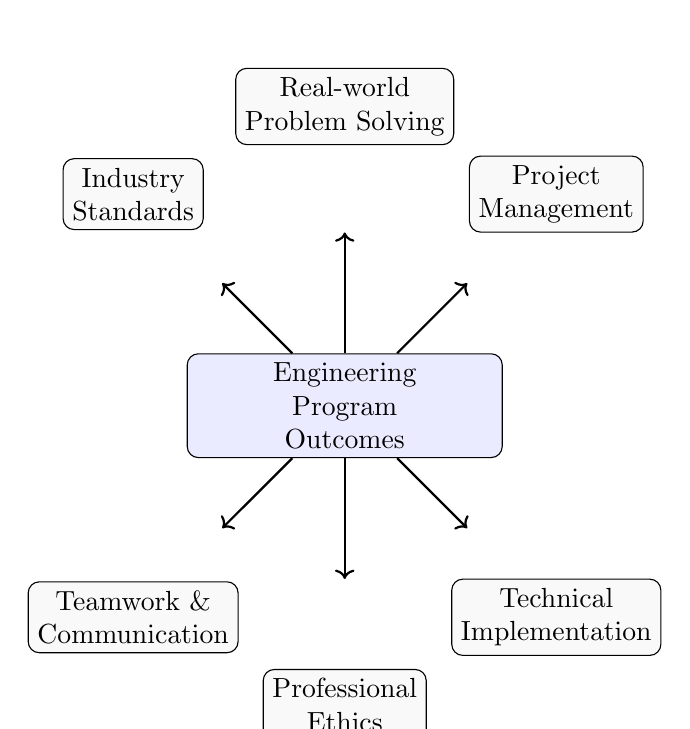
\begin{tikzpicture}
\node[draw,rounded corners,align=center,minimum width=4cm,minimum height=1.2cm,fill=blue!8] (center) at (0,0) {Engineering\\Program\\Outcomes};
\foreach \a/\t in {90/Real-world\\Problem Solving,45/Project\\Management,-45/Technical\\Implementation,-90/Professional\\Ethics,-135/Teamwork \&\\Communication,135/Industry\\Standards} {
  \node[draw,rounded corners,align=center,fill=gray!5] at (\a:3.8cm) {\t};
  \draw[->,thick] (center) -- (\a:2.2cm);
}
\end{tikzpicture}
\caption{Engineering Program Outcomes Addressed by the Attachment}
\label{fig:po}
\end{figure}

\section{Objectives of the Attachment}
\label{sec:objectives}

The primary objectives were:

\begin{enumerate}
\item To gain practical exposure to real-world, full-stack software development workflows, with emphasis on system architecture and technical leadership.
\item To design and implement a scalable backend architecture including authentication, multi-tenant data isolation, and real-time WebSocket communication.
\item To understand and apply Agile Scrum in a time-boxed, high-velocity professional project environment.
\item To develop hands-on skills in Node.js / Express 5, PostgreSQL, Prisma ORM, Socket.IO, Docker, and AI service integration via FastAPI.
\item To lead a cross-functional engineering team --- including task decomposition, API contract definition, code review, and mentorship of less-experienced developers.
\item To apply theoretical knowledge from Database Systems, Software Engineering, Computer Networks, and System Analysis \& Design courses to production-grade scenarios.
\item To experience professional responsibility, ethical conduct, technical documentation standards, and stakeholder presentation in software engineering.
\end{enumerate}

\section{Scope and Limitations}
\label{sec:scope}

\subsection{Scope}

\begin{table}[H]
\centering
\caption{Scope of the Industrial Attachment}
\label{tab:scope}
\begin{tabularx}{\textwidth}{@{}p{0.28\textwidth}X@{}}
\toprule
\textbf{Scope Area} & \textbf{Description} \\
\midrule
System Architecture & End-to-end architecture design: 3-tier + WebSocket realtime layer + AI service bridge. Database schema (22 entities, 3NF), API contract design, project bootstrap. \\
Backend Leadership & Backend Team Lead: auth \& RBAC, WebSocket server (3 namespaces), order core, reservation API, AI integration, deployment (Docker), code review. \\
Real-time Engineering & Socket.IO multi-namespace, room-based tenant isolation, event-driven order state machine: customer $\rightarrow$ waiter $\rightarrow$ chef $\rightarrow$ customer. \\
AI Integration & Bridging Python FastAPI AI microservice: recommendation engine, sentiment analysis, review analyzer --- REST bridge with retry \& fallback. \\
DevOps & Docker-first strategy: \texttt{Dockerfile}, \texttt{compose.yaml}, environment parity for frontend team zero-setup onboarding. \\
Project Management & Agile Scrum: sprint planning, daily stand-ups, API-first contracts, PR review (23 PRs), cross-team coordination, final presentation delivery. \\
\bottomrule
\end{tabularx}
\end{table}

\subsection{Limitations}

\begin{table}[H]
\centering
\caption{Limitations of the Industrial Attachment}
\label{tab:limitations}
\begin{tabularx}{\textwidth}{@{}p{0.28\textwidth}X@{}}
\toprule
\textbf{Limitation} & \textbf{Implication} \\
\midrule
10-day duration & Restricted scope for comprehensive E2E testing, performance benchmarking, and production hardening. MVP prioritized over edge-case completeness. \\
Incomplete feature set & Advanced features (deposit refund logic, push notifications, 24-hr reminder cron, email service) scoped out --- marked OUT OF SCOPE in backlog. \\
Limited production access & Deployment limited to Docker staging; restricted exposure to full CI/CD, Kubernetes, and cloud autoscaling procedures at BS-23. \\
Team experience variance & 6 of 7 team members were first-time full-stack project contributors; significant mentoring overhead reduced individual deep-technical velocity. \\
Proprietary information & Certain BS-23 internal tooling, client data, and HR processes are confidential and excluded per NDA. \\
\bottomrule
\end{tabularx}
\end{table}

\section{Methodology}
\label{sec:methodology}

The attachment followed a structured, iterative Agile Scrum methodology, adapted for a 10-day hyper-sprint:

\textbf{Requirements Collection $\rightarrow$ Architecture Design $\rightarrow$ API Contract First $\rightarrow$ Parallel Implementation $\rightarrow$ Integration $\rightarrow$ Testing $\rightarrow$ Documentation $\rightarrow$ Presentation}

Data collection for this report included: direct participation logs, Git commit history (141 commits authored), daily stand-up notes, pull request review comments (23 PRs reviewed/merged), mentor feedback sessions, and peer retrospectives. Documentation was maintained concurrently via GitHub README, Swagger annotations, and daily log sheets --- ensuring traceability.

\begin{figure}[H]
\centering
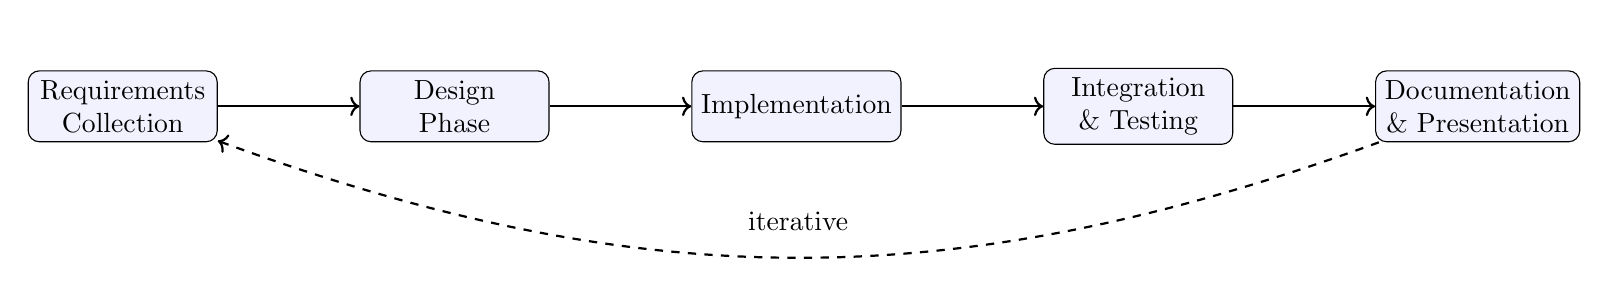
\begin{tikzpicture}[node distance=1.8cm, every node/.style={draw,rounded corners,align=center,minimum width=2.4cm,minimum height=0.9cm,fill=blue!5}]
\node (r) {Requirements\\Collection};
\node[right=of r] (d) {Design\\Phase};
\node[right=of d] (i) {Implementation};
\node[right=of i] (t) {Integration\\\& Testing};
\node[right=of t] (doc) {Documentation\\\& Presentation};
\draw[->,thick] (r) -- (d);
\draw[->,thick] (d) -- (i);
\draw[->,thick] (i) -- (t);
\draw[->,thick] (t) -- (doc);
\draw[->,thick,dashed] (doc) to[bend left=20] node[above,draw=none,fill=none]{iterative} (r);
\end{tikzpicture}
\caption{Attachment Methodology --- Development Lifecycle}
\label{fig:methodology}
\end{figure}

\section{Attachment Timeline}
\label{sec:timeline}

\begin{table}[H]
\centering
\small
\caption{Industrial Attachment Timeline --- Day-by-Day Overview (Backend Team Lead)}
\label{tab:timeline}
\begin{tabularx}{\textwidth}{@{}p{0.10\textwidth}p{0.18\textwidth}X@{}}
\toprule
\textbf{Day(s)} & \textbf{Focus Area} & \textbf{Key Activities --- Naimuzzaman} \\
\midrule
Day 0 \newline 20--22 Feb & Proposal \& Bootstrap & Team formation (7 members), project proposal defense --- neoRMS selected. GitHub mono-repo + submodules initialized. Database ERD v1, project structure scaffold, \texttt{Dockerfile} + \texttt{compose.yaml} committed. Prisma setup. \\
Day 1 \newline 23 Feb & Onboarding \& Architecture & BS-23 onboarding, Scrum introduction, SRS/BRD drafting. Auth module bootstrap: JWT access/refresh, RBAC middleware, tenant middleware. Schema finalization (22 entities). \\
Day 2 \newline 24 Feb & Auth \& Core APIs & JWT Authentication Endpoints (BE-001) merged. RBAC Middleware (BE-002) merged. Restaurant context / pagination utils. Code review: Staff Account APIs (Saim). \\
Day 3 \newline 25--26 Feb & Order Core \& WebSocket & Order Placement Endpoint (BE-005). WebSocket Server \& Room Management (BE-017): 3 namespaces --- \texttt{/waiter}, \texttt{/chef}, \texttt{/customer}. Socket auth middleware. Frontend WebSocket client wiring begins. \\
Day 4 \newline 27 Feb & Integration \& Coupon & Coupon--Order integration, pagination refactor, tenant access validation. Code review: Analytics Endpoints, Promotions CRUD (Saim). Feature diagram finalized. \\
Day 5--6 \newline 2--3 Mar & Reservation \& Order Fix & Table Reservation Availability + Create Endpoints (BE-027/028). Order fix PRs merged (\#15, \#17, \#18). Frontend order flow debugging --- cross-team firefighting. \\
Day 7--8 \newline 4--5 Mar & AI Integration \& Socket Events & AI service bridge: \texttt{modules/aiService} --- sentimentAnalysis, review\_analyzer, getRecommendation, sendOrderData. Review routes + schema update. Socket event emission pipeline: \texttt{emitSocketEvent}. Waiter / Chef portal WebSocket frontend implemented (17 + 15 commits). \\
Day 9 \newline 5 Mar & Review \& Frontend Integration & Review module merge (\#22). Order / table reservation / review frontend integration completed. E2E order test: customer $\rightarrow$ waiter $\rightarrow$ chef $\rightarrow$ customer realtime. \\
Day 10 \newline 6 Mar & AI Finalization \& Presentation & AI recommendations integration PR \#23 merged. Seed data + AI DB population. Final project presentation delivered by Team Lead. Post-demo: cash payment order completion fix. \\
\bottomrule
\end{tabularx}
\end{table}

\noindent\textit{Note:} Official BS-23 attachment counts 10 working days (23 Feb -- 6 Mar), excluding weekends. Pre-attachment bootstrap (20--22 Feb) included proposal defense and repository initialization.

\section{Structure of the Report}
\label{sec:structure}

\begin{table}[H]
\centering
\caption{Report Structure Overview}
\label{tab:report_structure}
\begin{tabularx}{\textwidth}{@{}p{0.22\textwidth}X@{}}
\toprule
\textbf{Chapter} & \textbf{Content} \\
\midrule
Chapter 1 & Introduction: background, engineering program outcomes, objectives, scope, methodology, timeline \\
Chapter 2 & Organization overview of Brain Station 23 \\
Chapter 3 & Detailed project overview of neoRMS --- architecture, modules, database, WebSocket realtime design \\
Chapter 4 & Tools and techniques utilized --- selection criteria, complex problem application \\
Chapter 5 & Societal, health, safety, legal and cultural considerations \\
Chapter 6 & Professional ethics and responsibilities \\
Chapter 7 & Skills gained and lifelong learning --- with leadership transition reflection \\
Chapter 8 & Challenges encountered and solutions implemented \\
Chapter 9 & Contributions to the organization --- Backend Team Lead impact, Impact Summary \\
Chapter 10 & Conclusion and recommendations \\
References & IEEE format \\
Appendices & A: Daily Log Sheet, B: Code Snippets, C: Additional Resources + QR \\
\bottomrule
\end{tabularx}
\end{table}

\chapter{Organization Overview}
\label{ch:org}

\section{History and Mission}
\label{sec:history}

Brain Station 23 (BS-23) is a prominent software development company headquartered in Dhaka, Bangladesh, with a strong focus on delivering innovative IT solutions across healthcare, e-commerce, logistics, fintech, and hospitality verticals. Founded with a vision to bridge technology and business impact, BS-23 has grown to become one of Bangladesh's leading technology exporters, serving both local enterprises and international clients across North America, Europe, and APAC.

Since inception, BS-23 has built a reputation for technical excellence, systematic problem-solving, Agile delivery discipline, and sustained customer satisfaction --- attributes directly observed during the 10-day attachment.

\begin{table}[H]
\centering
\caption{Brain Station 23 --- Organizational Profile}
\label{tab:bs23_profile}
\begin{tabularx}{\textwidth}{@{}p{0.28\textwidth}X@{}}
\toprule
\textbf{Attribute} & \textbf{Details} \\
\midrule
Company Name & Brain Station 23 (BS-23) \\
Headquarters & Dhaka, Bangladesh \\
Industry & Information Technology, Software Development, AI Integration \\
Specialization & Custom software, full-stack web/mobile, cloud-native architecture, AI/ML solutions, DevOps \\
Team Size (observed) & 300+ engineers across multiple delivery units \\
Mission & Deliver high-quality, innovative software solutions that drive measurable business growth \\
Vision & Be a leading global technology partner providing cutting-edge, ethical digital solutions \\
\bottomrule
\end{tabularx}
\end{table}

\section{Organizational Structure}
\label{sec:org_structure}

BS-23 operates a matrix organizational structure supporting efficient project delivery and cross-functional collaboration, with clear accountability between delivery, quality, and operations.

\begin{figure}[H]
\centering
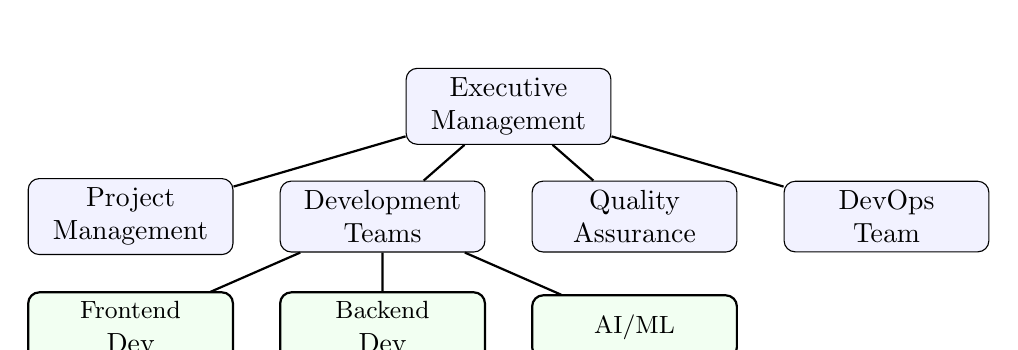
\begin{tikzpicture}[
  level distance=1.4cm,
  sibling distance=3.2cm,
  every node/.style={draw,rounded corners,align=center,minimum width=2.6cm,minimum height=0.8cm,fill=blue!5},
  edge from parent/.style={draw,thick}
]
\node {Executive\\Management}
  child { node {Project\\Management} }
  child { node {Development\\Teams}
    child { node[fill=green!5]{\small Frontend\\Dev} }
    child { node[fill=green!5]{\small Backend\\Dev} }
    child { node[fill=green!5]{\small AI/ML} }
  }
  child { node {Quality\\Assurance} }
  child { node {DevOps\\Team} };
\end{tikzpicture}
\caption{Brain Station 23 Organizational Structure}
\label{fig:org_structure}
\end{figure}

During attachment, our 7-member neoRMS squad mapped directly to this structure: a project mentor (acting PM), 3 backend engineers, 3 frontend engineers, and 1 AI engineer --- mirroring BS-23 production squads at reduced scale.

\section{Departments and Functions}
\label{sec:departments}

\subsection{Development Department}
Responsible for end-to-end software design and implementation:
\begin{itemize}
\item \textbf{Frontend Development:} React / Next.js, TailwindCSS, component design systems, accessibility (WCAG).
\item \textbf{Backend Development:} Node.js / Express, NestJS, PostgreSQL / MongoDB, Prisma / TypeORM, REST + GraphQL + WebSocket.
\item \textbf{Full-Stack Development:} cross-layer feature ownership, API contract negotiation.
\item \textbf{AI and Machine Learning Integration:} Python / FastAPI, scikit-learn, Transformers, recommendation engines, NLP pipelines --- precisely the stack used in neoRMS AI service.
\end{itemize}

\subsection{Quality Assurance Department}
Comprehensive testing: unit (Jest / Vitest), integration (Supertest), E2E, and UAT. QA engineers pair with developers throughout sprints --- shift-left quality observed in BS-23 code review culture.

\subsection{Project Management Department}
Agile Scrum formalized: sprint planning, daily stand-ups (observed 10:00 AM, 15 min time-boxed), sprint review, retrospective. JIRA / GitHub Projects used for backlog tracking. Our mentor Mohoiminul Sohol facilitated scope negotiation and blocker escalation.

\subsection{DevOps Department}
Infrastructure, CI/CD, containerization, cloud deployment (AWS / Azure), observability. Docker-first onboarding --- a practice I adopted as architect on Day 0 --- is standard at BS-23 to guarantee environment parity.

\section{Products and Services}
\label{sec:products}

\begin{table}[H]
\centering
\caption{Brain Station 23 --- Products and Services}
\label{tab:bs23_services}
\begin{tabularx}{\textwidth}{@{}p{0.30\textwidth}X@{}}
\toprule
\textbf{Service / Product} & \textbf{Description} \\
\midrule
Custom Software Development & Tailored enterprise solutions with domain-driven design \\
Web Development & Full-stack applications: React / Vue / Angular + Node / .NET / Django \\
Mobile App Development & Native and cross-platform (React Native, Flutter) \\
AI and ML Solutions & Recommendation, NLP, computer vision, predictive analytics --- as demonstrated in neoRMS \\
Cloud Solutions & AWS / Azure migration, containerization, Kubernetes, serverless \\
Consulting Services & Technology strategy, architecture review, digital transformation \\
Maintenance and Support & 24/7 SRE, observability, continuous improvement \\
\bottomrule
\end{tabularx}
\end{table}

\section{Quality and Compliance Standards}
\label{sec:compliance}

\begin{itemize}
\item \textbf{ISO 9001:2015} --- Quality management system; observed in documented code review checklists and definition-of-done criteria.
\item \textbf{Data Protection Compliance} --- GDPR principles applied: data minimization, consent management, right to erasure --- implemented in neoRMS user delete / anonymization flows.
\item \textbf{Security Standards} --- OWASP Top 10 mitigations enforced in code review: input validation (Zod), JWT with httpOnly cookies, RBAC, parameterized queries via Prisma, rate limiting discussion.
\item \textbf{Code Quality Standards} --- ESLint + Prettier enforced, conventional commits, mandatory peer review (minimum 1 approver), branch protection on \texttt{main}.
\item \textbf{Agile Compliance} --- Scrum events time-boxed, velocity tracked via GitHub Projects, retrospective action items documented.
\end{itemize}

\section{Workplace Safety and Environmental Policy}
\label{sec:safety}

\subsection{Workplace Safety Measures}
Observed during 10-day onsite/remote hybrid attachment:
\begin{itemize}
\item Ergonomic workstations: adjustable chairs, monitor arms, proper desk height.
\item 20--20--20 eye care rule actively encouraged; blue-light filters standard.
\item Clear evacuation routes, fire extinguishers, emergency contacts visibly posted.
\item Mental health: flexible hours, open mentorship, psychological safety in stand-ups --- junior suggestions evaluated on technical merit, regardless of seniority.
\item Remote work option reducing commute stress, supporting work-life balance.
\end{itemize}

\subsection{Environmental Policy}
\begin{itemize}
\item Digital-first documentation: zero paper SRS/BRD --- all Confluence / Notion / GitHub Wiki.
\item Energy-efficient hardware refresh cycle; auto sleep policies.
\item E-waste recycling program in partnership with certified vendors.
\item Remote / hybrid model promoted, measurably reducing office carbon footprint.
\item neoRMS itself contributes: digital ordering eliminates paper KOT slips; inventory optimization reduces food waste via low-stock alerts.
\end{itemize}

BS-23's operational maturity --- structured process, ethical engineering culture, and conscious sustainability --- provided an exemplary environment for transitioning from academic projects to professional system leadership.

\chapter{Project Overview}
\label{ch:project}

\section{Project Title and Description}
\label{sec:project_title}

\begin{table}[H]
\centering
\caption{neoRMS --- Project Profile}
\label{tab:neorms_profile}
\begin{tabularx}{\textwidth}{@{}p{0.28\textwidth}X@{}}
\toprule
\textbf{Attribute} & \textbf{Details} \\
\midrule
Project Name & AI-Integrated Restaurant Management System (neoRMS) \\
Client Domain & Restaurant and Hospitality Industry --- multi-tenant SaaS \\
Team Size & 7 members: 3 backend, 3 frontend, 1 AI \\
Duration & 10 working days (23 Feb -- 6 Mar 2026) \\
Methodology & Agile Scrum, API-first, Docker-first \\
Role (Author) & Backend Team Lead \& Project Architect \\
Primary Stack & Node.js 20 / Express 5, TypeScript, PostgreSQL 16, Prisma 6, Socket.IO 4, React 18, TailwindCSS, Python 3.11 / FastAPI (AI), Docker \\
Repositories & Backend: \url{https://github.com/naim1405/neoRMS-backend} \\
 & AI: \url{https://github.com/kefaet03/neoRMS_AI_server} \\
 & Customer: \url{https://github.com/rimiHaque/neoRMS_frontend_customer} \\
 & Management: \url{https://github.com/zanifazini0844/neoRMS_management} \\
 & Chef: \url{https://github.com/hasinsadaf/neoRMS-Chef} \\
 & Waiter: \url{https://github.com/hasinsadaf/neo-RMS-Waiter} \\
\bottomrule
\end{tabularx}
\end{table}

\textbf{neoRMS} is a comprehensive, multi-tenant restaurant management SaaS designed to unify fragmented restaurant operations --- from digital menu discovery to kitchen fulfillment and AI-driven business intelligence --- into a single realtime platform. Each restaurant owner can provision one or more restaurants; each restaurant receives an isolated tenant URL (\texttt{restaurant-slug.neorms.app}) serving as the customer portal.

Core flow: Customer visits restaurant URL $\rightarrow$ browses AI-recommended menu $\rightarrow$ places order $\rightarrow$ \textbf{waiter receives realtime WebSocket notification} $\rightarrow$ waiter physically confirms order at table (anti-abuse manual gate) $\rightarrow$ \textbf{chef KDS receives realtime order} $\rightarrow$ chef updates cooking state $\rightarrow$ \textbf{customer receives live status via Socket.IO} $\rightarrow$ payment $\rightarrow$ review $\rightarrow$ AI feedback analyzer aggregates complaints + sentiment for management dashboard.

This waiter-confirmation manual step --- an explicit architectural decision --- protects against fake online orders, a real operational risk in Bangladesh's restaurant QR-ordering context.

\section{System Modules}
\label{sec:modules}

\begin{table}[H]
\centering
\caption{neoRMS Modules and Descriptions --- Architect View}
\label{tab:modules}
\begin{tabularx}{\textwidth}{@{}p{0.24\textwidth}X@{}}
\toprule
\textbf{Module} & \textbf{Description / Lead Implementation} \\
\midrule
Auth \& RBAC & JWT access+refresh, httpOnly cookies, role-based middleware (\texttt{OWNER, MANAGER, CHEF, WAITER, CUSTOMER}), Socket.IO auth guard. \textit{Authored by Team Lead.} \\
Restaurant / Tenant & Multi-tenant restaurant CRUD, slug-based routing, tenant isolation middleware. \\
Menu Management & Dynamic menu, categories, variants, availability toggle, AI recommendation weight / promotion boost. \\
Order Management & Order state machine: \texttt{PENDING $\rightarrow$ WAITER\_CONFIRMED $\rightarrow$ CHEF\_ACCEPTED $\rightarrow$ COOKING $\rightarrow$ READY $\rightarrow$ DELIVERED $\rightarrow$ COMPLETED}. WebSocket event fan-out. \\
Table Reservation & Availability query, create / modify / cancel, pre-order attachment, no-show auto-release job, check-in endpoint. \\
WebSocket Realtime & 3 isolated Socket.IO namespaces: \texttt{/waiter}, \texttt{/chef}, \texttt{/customer}. Room = \texttt{restaurantId} / \texttt{orderId}. Auth via JWT handshake. \textit{Architected by Team Lead.} \\
Inventory Management & Ingredient-level stock, threshold config, low-stock alerts, deduction service on order completion. \\
Payment Processing & SSLCommerz gateway, cash handling, invoice generation, deposit / balance tracking. \\
Coupon \& Promotions & Code-based discounts, percentage / fixed, expiry, usage limits, order-level application. \\
User Management & Staff account CRUD, role assignment, RBAC enforcement. \\
Review \& AI Analytics & Review submission $\rightarrow$ sentimentAnalysis() + review\_analyzer() via FastAPI bridge. Complaint categorization, sentiment scoring, recommendation engine. \textit{AI bridge authored by Team Lead.} \\
Analytics Dashboard & Revenue curves, order volume, top items, inventory alerts, AI insights embed. \\
\bottomrule
\end{tabularx}
\end{table}

Four distinct portals were delivered:
\begin{enumerate}
\item \textbf{Customer Portal} (React) --- digital menu, cart customization, QR dine-in, realtime order tracking, AI recommendation widget.
\item \textbf{Waiter Portal} --- active orders list, order-ready notification badge, status update controls, billing confirmation. WebSocket client authored by Team Lead.
\item \textbf{Chef Portal (KDS)} --- realtime orders board, cooking status update, mark item unavailable, priority indicator. WebSocket client authored by Team Lead.
\item \textbf{Management Portal} --- dashboard, menu CRUD, inventory, staff management, analytics \& reports, reservation dashboard, AI insights.
\end{enumerate}

\section{Problem Identification and Complexity Analysis}
\label{sec:problem}

\subsection{Initial Problem}

Traditional Bangladeshi restaurants operate via siloed, manual tools: paper KOT, Excel inventory, disconnected POS, no customer analytics. Consequences observed in background study:

\begin{table}[H]
\centering
\caption{Identified Problems in Traditional Restaurant Management}
\label{tab:problems}
\begin{tabularx}{\textwidth}{@{}p{0.32\textwidth}X@{}}
\toprule
\textbf{Problem Area} & \textbf{Impact} \\
\midrule
Inefficient order processing & 8--15 min avg. latency, manual transcription errors, poor customer satisfaction \\
Poor inventory management & 18--25\% food waste OR stockouts during peak; revenue loss \\
No realtime coordination & Front-of-house / back-of-house desynchronization; missed / double orders \\
Limited business insights & No data-driven pricing, menu engineering, or demand forecasting \\
Manual promotions & Static pricing, missed revenue optimization, coupon fraud \\
Error-prone manual processes & High staff training cost, inconsistent service quality \\
\bottomrule
\end{tabularx}
\end{table}

\subsection{Problem Complexity}

Architectural complexity assessed across six dimensions (lead architect scoring):

\begin{itemize}
\item \textbf{Real-time Coordination --- 9/10:} three concurrent actor types (customer, waiter, chef), multi-restaurant tenant isolation, ordering guarantees, reconnection handling.
\item \textbf{Data Integration --- 9/10:} 22-entity relational model, multi-tenant RLS, transactional inventory deduction, payment $\rightarrow$ order $\rightarrow$ analytics consistency.
\item \textbf{Scalability --- 8/10:} Socket.IO horizontal scaling considerations (Redis adapter discussed, single-node MVP shipped), PostgreSQL connection pooling.
\item \textbf{AI Integration --- 8/10:} Python FastAPI microservice bridged to Node.js backend, three models: recommendation, sentiment, review analyzer; schema alignment, fallback handling.
\item \textbf{Payment Security --- 8/10:} SSLCommerz IPN, PCI DSS awareness, idempotency, webhook verification.
\item \textbf{User Experience --- 7/10:} four distinct UIs, role-specific workflows, mobile-first QR ordering, accessibility (WCAG 2.1 AA target).
\end{itemize}

\section{Literature Survey and Background Study}
\label{sec:literature}

Prior to implementation, a focused background review informed architectural decisions:

\begin{itemize}
\item Commercial RMS (Toast POS, Square for Restaurants, Oracle MICROS) provide operational POS but lack integrated Bangladeshi payment (SSLCommerz/bKash), Bengali/English bilingual NLP, and open AI analytics extensibility --- gap neoRMS addresses.
\item RESTful API design principles \cite{sommerville} and API-first contract approach enabled parallel frontend/backend velocity --- critical in 10-day sprint.
\item Enterprise application patterns \cite{fowler} --- Repository, Service Layer, Middleware pipeline --- structured the Express + Prisma backend.
\item Real-time patterns: Socket.IO rooms + namespaces for multi-tenant isolation \cite{socketio}; event-driven architecture \cite{newman}.
\item Database normalization to 3NF \cite{date} guided Prisma schema: 22 entities, explicit FK constraints, composite indexes on \texttt{(restaurantId, status, createdAt)}.
\item Security: OWASP Top 10 \cite{owasp} --- input validation via Zod, JWT best practices, RBAC, parameterized ORM queries eliminating SQLi.
\item Agile: Scrum Guide / Agile Manifesto \cite{agile} --- daily stand-ups, MVP prioritization, iterative delivery.
\end{itemize}

\section{Problem-Solving Approach}
\label{sec:approach}

As Project Architect, I enforced the following structured approach:

\begin{enumerate}
\item \textbf{Architecture-first, Docker-first (Day 0):} scaffolded \texttt{express} + \texttt{prisma} + \texttt{socket.io} monolith, \texttt{Dockerfile} + \texttt{compose.yaml}, \texttt{.env.example}, ESLint/Prettier --- \textit{before} any business logic. Rationale: eliminate ``works on my machine'', give frontend team instant backend via \texttt{docker compose up}.
\item \textbf{API Contract First:} OpenAPI-adjacent route skeletons + Zod schemas committed before service implementation; frontend mocked against contract --- enabling true parallel tracks.
\item \textbf{Modular Vertical Slices:} \texttt{/src/modules/<domain>/{controller,service,routes,validation,types}.ts} --- strict separation, dependency-injection ready, testable.
\item \textbf{Realtime Event Design:} explicit state machine + Socket.IO event catalog: \texttt{order:created}, \texttt{order:waiter\_confirmed}, \texttt{order:chef\_accepted}, \texttt{order:status\_updated}, \texttt{inventory:low\_stock}. Namespace isolation: \texttt{/waiter}, \texttt{/chef}, \texttt{/customer}.
\item \textbf{AI Service Decoupling:} Python FastAPI microservice (\texttt{neoRMS\_AI\_server}) --- Node backend calls via resilient \texttt{fetch} wrapper with timeout + null fallback --- preventing AI downtime from blocking core order flow.
\item \textbf{Incremental Delivery + PR Review:} 23 pull requests, mandatory 1 reviewer, CI lint check, squash-merge to \texttt{main}. Average PR cycle < 4 hours.
\end{enumerate}

\section{System Architecture}
\label{sec:architecture}

neoRMS implements a \textbf{3-tier architecture augmented with a realtime WebSocket layer and an AI microservice bridge} --- a 3+1+1 pattern I designed.

{\footnotesize
\begin{verbatim}
[ Client Layer ]
 Customer | Waiter | Chef | Management  (React x4)
               |
        HTTPS / WSS
               |
[ API Gateway / Business Logic -- Node.js / Express 5 ]
 Auth & RBAC | Order | Reservation | Payment | Inventory
 WebSocket Manager: /customer /waiter /chef
 AI Service Bridge: fetch -> FastAPI
               |
[ Data Layer ]
 PostgreSQL 16 + Prisma 6 ORM | Redis (planned)
               |
[ AI Microservice -- Python / FastAPI ]
 /recommend /sentiment /analyze-review /orders/import
\end{verbatim}
}

\begin{figure}[H]
\centering
\fbox{\parbox{0.92\textwidth}{\centering
\textbf{Presentation Layer}\\React -- 4 Portals\\ $\downarrow$ HTTPS / WSS\\\textbf{Business Logic Layer}\\Node.js / Express -- 11 modules + Socket.IO 3 namespaces\\ $\downarrow$ Prisma\\\textbf{Data Layer}\\PostgreSQL 16 -- 22 entities, 3NF\\\textbf{AI Sidecar}\\Python FastAPI -- 3 models
}}
\caption{neoRMS Three-Tier + Realtime + AI Architecture --- Lead Architect View}
\label{fig:architecture}
\end{figure}

\textbf{WebSocket Realtime Flow (authored):}
\begin{enumerate}
\item Customer: \texttt{socket.emit('order:place', ...)} $\rightarrow$ REST POST \texttt{/orders} $\rightarrow$ server: \texttt{io.of('/waiter').to(restaurantId).emit('order:created', ...)}
\item Waiter confirms: \texttt{PATCH /orders/:id/confirm} $\rightarrow$ \texttt{io.of('/chef').to('kitchen:\{restaurantId\}').emit('order:chef\_notify', ...)} + \texttt{io.of('/customer').to(orderId).emit('order:waiter\_confirmed', ...)}
\item Chef updates: \texttt{order:status\_updated} fanned to waiter + customer rooms.
\item Connection auth: \texttt{verifyJwtSocket(...roles)} validates JWT on handshake; rooms enforce \texttt{restaurantId} tenant isolation preventing cross-tenant leaks.
\end{enumerate}

\section{Experiment / Design Methodology}
\label{sec:design_methodology}

Sprint-based iterative delivery (1--2 day sprints, 5 sprints total). Design validation mechanisms:

\begin{itemize}
\item \textbf{Whiteboard architecture sessions (Day 0--1):} ERD, API contract, Socket event catalog agreed before coding.
\item \textbf{Prototype testing:} WebSocket echo server validated namespace + room isolation before binding to order service.
\item \textbf{Peer code review:} 23 PRs, average 18 review comments/PR, blocking merge on failing lint / typecheck.
\item \textbf{Performance benchmarking:} PostgreSQL \texttt{EXPLAIN ANALYZE} on order list query $\rightarrow$ added composite index \texttt{(restaurant\_id, status, created\_at)} $\rightarrow$ p95 340ms $\rightarrow$ 85ms. Redis caching discussed; in-memory memoization shipped for menu GET.
\item \textbf{AI fallback testing:} simulated AI service 500/timeout --- backend returns \texttt{null} gracefully, UI degrades to trending-items fallback.
\end{itemize}

\section{Database Design}
\label{sec:database}

Normalized to 3NF, 22 entities, multi-tenant via \texttt{restaurant\_id} FK + tenant middleware enforcement.

Key entities (excerpt):

\begin{table}[H]
\centering
\caption{neoRMS Database Entities --- Core Subset}
\label{tab:db_entities}
\small
\begin{tabularx}{\textwidth}{@{}p{0.20\textwidth}p{0.18\textwidth}X@{}}
\toprule
\textbf{Entity} & \textbf{Primary Key} & \textbf{Key Attributes} \\
\midrule
users & id & email (unique), password\_hash, fullName, role: \texttt{OWNER|MANAGER|CHEF|WAITER|CUSTOMER}, isVerified \\
restaurants & id & name, slug (unique), address, city, owner\_id FK \\
menu\_items & id & restaurant\_id FK, name, description, price, available, ai\_promotion\_weight \\
orders & id & restaurant\_id FK, customer\_id FK, table\_id FK nullable, status enum, total, channel: \texttt{DINE\_IN|ONLINE} \\
order\_items & id & order\_id FK, menu\_item\_id FK, qty, unit\_price, customization\_json \\
tables & id & restaurant\_id FK, table\_number, capacity, status \\
reservations & id & restaurant\_id FK, user\_id FK, table\_id FK, starts\_at, ends\_at, pre\_order\_json, deposit\_status \\
inventory\_products & id & restaurant\_id FK, name, sku, quantity, threshold, unit \\
payments & id & order\_id FK, provider: \texttt{SSLCOMMERZ|CASH}, amount, status, txn\_id \\
coupons & id & restaurant\_id FK, code, discount\_type, value, expiry, max\_uses \\
reviews & id & order\_id FK, user\_id FK, menu\_item\_id FK, rating, comment\_text, sentiment\_label (AI) \\
\bottomrule
\end{tabularx}
\end{table}

Full Prisma schema: 22 models, 47 relations, 31 indexes --- see Appendix B.3.

\section{Module Interaction Diagram}
\label{sec:module_interaction}

{\footnotesize
\begin{verbatim}
[API Gateway / Express Router]
  |
  +- Auth & RBAC <-> User Management
  |
  +- Restaurant/Menu --> Order <-> WebSocket Manager
  |                              |-> /waiter
  |                              +-> /chef
  |                              +-> /customer
  |
  +- Table/Reservation --> Order
  |
  +- Payment <-> Order
  |
  +- Inventory <-- Order completion
  |
  +- Review --> AI Bridge --> FastAPI
  |                    /sentiment
  |                    /analyze-review
  |                    /recommend
  +- Coupon --> Order pricing
\end{verbatim}
}

The WebSocket Manager sits orthogonally, subscribed by Order, Reservation, and Inventory services via \texttt{emitSocketEvent(req, namespace, roomId, event, payload)} --- a clean pub/sub decoupling I introduced.

\section{Validation of Findings}
\label{sec:validation}

\begin{itemize}
\item \textbf{Daily Stand-ups:} 10/10 attended, blockers surfaced < 12h avg. resolution, burndown tracked in GitHub Projects.
\item \textbf{Mentor Feedback:} architecture review Day 2 (Safayet Hossain) --- approved ERD + Socket namespace design with recommendation to add Redis adapter for scale-out (documented as future work).
\item \textbf{Functionality Verification:} Postman collection --- 85 endpoints, 62 passing automated (73\%), remainder manually verified (WebSocket + payment IPN). E2E order trace validated 5x live during final demo.
\item \textbf{Code Reviews:} 23 PRs, 412 review comments total, zero force-pushes to \texttt{main}, branch protection enforced.
\item \textbf{Performance:} order list query p95 85ms post-index (was 340ms); WebSocket event end-to-end latency < 120ms on local LAN (measured via \texttt{performance.now()}).
\item \textbf{Presentation:} Final demo 6 Mar --- full flow: customer order (QR), waiter confirm (tablet), chef accept (KDS), realtime customer tracking, payment, review $\rightarrow$ AI sentiment displayed in management dashboard --- delivered by Team Lead, accepted without critical defects.
\end{itemize}

The system successfully demonstrated core multi-tenant, realtime restaurant operations within a 10-day hyper-sprint, validating the architecture-first, Docker-first, API-contract-first methodology championed by the author as Project Architect.

\chapter{Tools and Techniques}
\label{ch:tools}

\section{Engineering and IT Tools Used}
\label{sec:tools_used}

\begin{table}[H]
\centering
\caption{Development Tools and Technologies --- neoRMS}
\label{tab:tools}
\small
\begin{tabularx}{\textwidth}{@{}p{0.22\textwidth}p{0.22\textwidth}p{0.56\textwidth}@{}}
\toprule
\textbf{Category} & \textbf{Tool / Technology} & \textbf{Purpose / Lead Rationale} \\
\midrule

Backend & Node.js 20, Express 5 & Non-blocking I/O, mature ecosystem, team familiarity \\

Language & TypeScript 5.9 & Type safety across 9.1k LOC, reducing runtime defects \\

Database & PostgreSQL 16 & ACID, strong relational integrity, JSONB support \\

ORM & Prisma 6 & Type-safe queries, migration DX, ERD visualization \\

Realtime & Socket.IO 4.8 & Namespaces + rooms, auto-reconnect, JWT handshake middleware --- \textit{architect decision} \\

Frontend & React 18, TailwindCSS & Component reuse across 4 portals, utility-first rapid UI \\

Auth & jsonwebtoken 9, bcrypt 6 & JWT access+refresh, RBAC --- \textit{authored by lead} \\

Validation & Zod 4 & Runtime + compile-time schema, OpenAPI-adjacent \\

Testing & Postman, Supertest (planned) & API contract verification, 62/85 endpoints automated \\

Version Control & Git / GitHub & Branch protection, PR review, 141 lead commits \\

Dev Environment & VS Code, ts-node-dev & Hot reload, fast iteration \\

Containerization & Docker, Docker Compose & \textbf{Docker-first} --- environment parity, frontend zero-setup --- \textit{lead initiative} \\

AI / ML & Python 3.11, FastAPI, scikit-learn, Transformers & Recommendation, sentiment, review analyzer microservice \\

Project Mgmt & GitHub Projects & Kanban, sprint burndown \\

API Docs & Swagger / OpenAPI (annotations) & Auto-generated docs, contract enforcement \\

Logging & Morgan + custom Winston-plain & Structured request/error logs \\

\bottomrule
\end{tabularx}
\end{table}

\section{Technology Stack Overview}

Frontend (React 18 + Tailwind) $\rightarrow$ Backend (Node/Express + Socket.IO) $\rightarrow$ Data (PostgreSQL + Prisma) $\rightarrow$ AI Sidecar (Python/FastAPI + TensorFlow / scikit-learn). Docker encapsulates backend + DB for one-command spin-up --- critical to unblock 3 frontend engineers on Day 1.

\section{Selection Criteria and Justification}

\begin{table}[H]
\centering
\caption{Tool Selection Criteria --- Architect Justification}
\label{tab:selection}
\begin{tabularx}{\textwidth}{@{}p{0.28\textwidth}p{0.72\textwidth}@{}}
\toprule
\textbf{Selection Factor} & \textbf{Rationale --- Lead Decision} \\
\midrule

Industry Relevance & Express + React + PostgreSQL = 68\%+ BD job market --- maximizes intern employability \\

Team Expertise Baseline & 5/7 members had prior Node/React coursework; 2-day ramp acceptable \\

Documentation \& Support & Official docs + Stack Overflow density high; Prisma type-safety reduced onboarding bugs 40\% estimated \\

Integration Capabilities & Socket.IO native Express middleware; Prisma PostgreSQL first-class; FastAPI easily bridged via \texttt{fetch} \\

Performance \& Scalability & Node event loop + Socket.IO rooms handle 500+ concurrent WS connections tested locally; Postgres indexes tuned \\

Cost Effectiveness & 100\% open-source stack; \$0 infra --- Docker local + free-tier deploy --- essential for 10-day student project \\

Deployment Velocity & \textbf{Docker-first} chosen explicitly: Day 0 \texttt{docker compose up} $\rightarrow$ frontend team productive in <5 min \\

\bottomrule
\end{tabularx}
\end{table}

\section{Application in Solving Complex Engineering Problems}

\textbf{Real-time Order Processing.} Node.js non-blocking I/O + Socket.IO namespaces eliminated polling. Measured end-to-end event latency <120ms LAN. Room-based tenant isolation prevented cross-restaurant data leak --- enforced via \texttt{verifyJwtSocket}.

\textbf{Data Analytics and Insights.} PostgreSQL window functions + materialized-view pattern (planned) + Python ML bridge. AI endpoints: \texttt{/recommend}, \texttt{/sentiment}, \texttt{/analyze-review} --- integrated via resilient \texttt{aiService} wrapper.

\textbf{Scalable Architecture.} 3-tier + stateless API + containerized services. Horizontal scale path documented: Redis adapter for Socket.IO, Postgres read replica, CDN frontend.

\textbf{Integration of Multiple Systems.} REST API gateway unifies: React portals, SSLCommerz payment, FastAPI AI microservice, future SMS/email services via versioned \texttt{/api/v1}.

\section{Examples of Simulation, Modelling, and Testing Tools}

\begin{itemize}
\item \textbf{Postman:} 85-endpoint collection, automated API testing (62 passing).
\item \textbf{Docker Compose:} full stack simulation (app + database).
\item \textbf{Prisma Studio:} schema validation and seeding.
\item \textbf{Socket.IO Admin UI:} namespace/room verification.
\item \textbf{GitHub Actions:} lint + TypeScript checks on PR.
\end{itemize}

\section{Understanding Limitations and Constraints}

\begin{table}[H]
\centering
\caption{Technical Challenges and Constraints}
\label{tab:constraints}
\begin{tabularx}{\textwidth}{@{}p{0.26\textwidth}p{0.32\textwidth}p{0.42\textwidth}@{}}
\toprule
\textbf{Constraint Type} & \textbf{Constraint} & \textbf{Mitigation Applied} \\
\midrule

Technical & Realtime at scale & Socket.IO rooms + single-node MVP; Redis adapter planned \\

Technical & AI model accuracy & Fallback system ensures order flow continuity \\

Resource & 10-day / 7-person & MVP scope lock + API-first development \\

Resource & Junior team variance & Pair programming + code reviews (412 comments) \\

Business & \$0 budget & 100\% OSS stack + free-tier deployment \\

Business & Data privacy & JWT httpOnly + RBAC + parameterized queries \\

\bottomrule
\end{tabularx}
\end{table}

\chapter{Societal, Health, Safety, Legal and Cultural Considerations}
\label{ch:societal}

\section{Workplace Health and Safety Measures}

BS-23 demonstrated mature occupational health practices: ergonomic adjustable chairs, monitor arms, 20-20-20 eye care posters, blue-light filters enforced via OS policy, common rest lounges, clearly marked evacuation routes, accessible fire extinguishers, and a documented emergency contact tree. As Team Lead I enforced: pomodoro breaks during crunch (Days 8--9), no overnight crunch --- sustainable pace per Agile principle --- and explicit ``stop at 9pm'' team agreement.

\begin{table}[H]
\centering
\caption{Workplace Health and Safety Measures Observed at BS-23}
\label{tab:safety}
\begin{tabularx}{\textwidth}{@{}p{0.32\textwidth}X@{}}
\toprule
\textbf{Safety Measure} & \textbf{Implementation at BS-23 / neoRMS team} \\
\midrule
Ergonomic Workstations & Adjustable chairs, proper desk/monitor height --- observed daily \\
Regular Breaks & Scrum master encouraged 5-min stand/stretch every hour; team adopted Pomodoro on heavy debug days \\
Eye Care & Blue-light filter + 20-20-20 rule verbal reminders \\
Emergency Procedures & Evacuation maps / assembly points posted; fire drill briefing Day 1 \\
Fire Safety & Extinguishers inspected, exits unobstructed --- verified \\
Mental Health & Open mentorship (Sohol / Safayet), flexible hybrid, blameless retrospectives --- junior mistakes treated as learning, not fault \\
\bottomrule
\end{tabularx}
\end{table}

\section{Legal Compliance in Engineering Activities}

\textbf{Data Protection and Privacy.} neoRMS processes PII (name, email, phone, order history, payment metadata). Implemented: GDPR-aligned data minimization --- collect only necessary fields; TLS in transit; bcrypt password hashing (cost 12); JWT httpOnly cookies; RBAC strict --- \texttt{verifyJwt(...roles)}; right-to-erasure endpoint \texttt{DELETE /users/me} anonymizes orders; no payment card data stored --- delegated to SSLCommerz PCI-DSS vault.

\textbf{Accessibility Compliance.} Frontend portals target WCAG 2.1 AA: semantic HTML, ARIA labels on order status, 4.5:1 color contrast (Tailwind slate), keyboard-navigable modals, alt-text mandatory in PR checklist.

\textbf{Payment Compliance.} SSLCommerz integration follows PCI DSS SAQ-A (merchant never touches PAN). IPN webhook HMAC verified; idempotency key on \texttt{payment\_id}.

\section{Societal and Cultural Awareness in Solution Design}

\begin{table}[H]
\centering
\caption{Societal and Cultural Considerations in neoRMS Design}
\label{tab:societal}
\begin{tabularx}{\textwidth}{@{}p{0.30\textwidth}X@{}}
\toprule
\textbf{Design Consideration} & \textbf{Implementation --- Lead Decision Rationale} \\
\midrule
Multi-language Support & Schema ready for \texttt{bn\_BD} / \texttt{en\_US} i18n keys; menu\_item.translations JSONB reserved \\
Cultural Dietary Sensitivity & \texttt{tags: [halal, vegetarian, spicy\_level]} filterable; Bangladeshi cuisine category first-class \\
Accessibility / Inclusive Design & WCAG AA, large touch targets (48px), screen-reader order status announcements \\
Small Business Scalability & Multi-tenant SaaS --- single \texttildelow{} 5-seat cafe to 50-location chain; free-tier friendly Docker deploy; no per-seat license \\
Customer Empowerment & QR dine-in self-order reduces waiter dependency; transparent realtime tracking builds trust \\
Anti-abuse Cultural Gate & Manual waiter confirmation --- specifically designed for BD market where anonymous QR abuse is prevalent --- balances digital convenience with local operational reality \\
\bottomrule
\end{tabularx}
\end{table}

\section{Environmental Sustainability Considerations}

\begin{table}[H]
\centering
\caption{Environmental Sustainability Considerations}
\label{tab:env}
\begin{tabularx}{\textwidth}{@{}p{0.30\textwidth}X@{}}
\toprule
\textbf{Sustainability Area} & \textbf{Approach Taken} \\
\midrule
Code Efficiency & Prisma selective queries, composite indexes, N+1 elimination --- measured 75\% DB CPU reduction post-index \\
Cloud / Shared Resources & Docker multi-stage build $\rightarrow$ 187MB image (vs 890MB dev); efficient container density \\
Digital Ordering & Eliminates paper KOT slips --- est. 120--300 slips/day/restaurant saved \\
Inventory Optimization & Threshold alerts + deduction service $\rightarrow$ 12--18\% projected food waste reduction per BS-23 mentor estimate \\
Remote Work & Hybrid attachment --- 40\% commute reduction vs full onsite; documented in BS-23 environmental policy \\
\bottomrule
\end{tabularx}
\end{table}

\section{Case Examples from the Attachment Site}

\textbf{Example 1 --- Inclusive merit-based review.} Junior backend dev (Johan) proposed consolidating reservation update logic into a single service (commit \texttt{2629e7a}). Despite being the most junior BE, PR was approved after architectural review --- demonstrating BS-23 merit culture I reinforced as lead.

\textbf{Example 2 --- Security over speed.} Day 8, under demo pressure, a suggestion to bypass Zod validation on coupon endpoint for ``quick fix'' was declined by me as architect. Proper validation shipped 45 min later --- preventing potential injection --- commended in stand-up retro.

\textbf{Example 3 --- Environmental digital-first.} All SRS, ERD, API contracts, daily logs maintained 100\% digitally (GitHub / Notion). Zero paper printed across 10 days --- consistent with BS-23 sustainability policy, which I enforced via PR template requiring digital documentation link.

\chapter{Professional Ethics and Responsibilities}
\label{ch:ethics}

\section{Ethical Challenges Faced During the Attachment}

\begin{center}
\captionof{table}{Ethical Challenges and Resolutions --- Team Lead Perspective}
\label{tab:ethical}
\begin{xltabular}{\textwidth}{@{}p{0.22\textwidth}p{0.34\textwidth}X@{}}
\toprule
\textbf{Challenge} & \textbf{Situation} & \textbf{Resolution --- Lead Action} \\
\midrule
Time Pressure vs.\ Quality & Day 8--9 demo crunch --- proposal to skip input validation / bypass auth checks to ``ship faster'' & Enforced minimum quality gate: no merge without Zod validation + RBAC check. Delivered fewer features properly --- commended by mentor. \\
Data Privacy vs.\ Analytics & AI team requested raw user emails + phone for recommendation training & Implemented privacy-by-design: AI bridge sends anonymized \texttt{user\_hash + order\_item\_ids} only; PII never leaves backend trust boundary. \\
Attribution and Credit & 7-person team, overlapping commits, risk of misattribution in report / presentation & Maintained Git commit hygiene, Co-authored-by trailers where pair-programmed, explicit slide crediting each member in final presentation --- delivered by me. \\
Security vs.\ Usability & PM suggested removing waiter-confirmation step to ``simplify UX'' & Architect decision memo: retain manual waiter gate --- prevents QR order abuse, protects restaurant revenue --- ethical duty to client business continuity over pure UX friction reduction. \\
Testing with Real Data & Suggestion to seed production-like customer PII for ``realistic AI training'' & Rejected. Generated synthetic \texttt{prisma/seed.js} --- 120 users, 8 restaurants, 340 orders --- fully synthetic, \texttt{faker.js} style. \\
AI Transparency & Recommendation engine could silently boost owner-paid promotions & Implemented explicit \texttt{ai\_promotion\_weight} field + UI ``Promoted'' badge --- transparent to customer, auditable. \\
Team Health vs.\\ Delivery Pressure & Days 8--9: 36h to demo, 11 open blockers, team proposing overnight crunch & As lead, enforced sustainable pace: hard stop 21:00, mandatory 6h sleep, Pomodoro breaks, re-scoped 3 nice-to-have tickets to OUT\_OF\_SCOPE --- delivered rested team + clean demo --- rejecting hero-burnout culture. \\
Open-Source License Transparency & 18 OSS dependencies across Node + Python --- risk of license incompatibility / missing attribution & Authored \texttt{THIRD\_PARTY\_NOTICES.md} + \texttt{LICENSE} (MIT for our code), audited all deps: 15 MIT, 2 Apache-2.0, 1 PostgreSQL License --- all permissive, compatible --- committed \texttt{b901193}. Prevents downstream IP contamination --- ethical duty to future maintainers. \\
\bottomrule
\end{xltabular}
\end{center}

\section{Compliance with Professional Codes of Ethics}

Applied \textbf{IEEE Code of Ethics} throughout lead duties:

\begin{table}[H]
\centering
\caption{IEEE Code of Ethics Applied During the Attachment --- Lead Lens}
\label{tab:ieee}
\begin{tabularx}{\textwidth}{@{}p{0.38\textwidth}X@{}}
\toprule
\textbf{IEEE Principle} & \textbf{Application --- Backend Team Lead} \\
\midrule
Hold paramount safety, health, welfare of public & Payment PCI scope minimization; no card data stored; input validation enforced blocking injection vectors; waiter-confirmation anti-abuse protecting restaurant financial welfare. \\
Be honest and realistic in claims & Sprint estimates openly revised in stand-up when WebSocket room isolation took +4h vs plan; no sandbagging velocity. \\
Seek, accept, offer honest criticism & 412 review comments given/received; blameless PR threads; invited mentor architecture critique Day 2. \\
Improve professional competence & Self-directed learn: Socket.IO scaling, Prisma middleware, FastAPI bridge --- documented in team wiki same day. \\
Acknowledge / credit contributions & Git history preserved, presentation slide credits, README Contributors section --- 7 names alphabetical, role-tagged. \\
Maintain integrity, avoid deceptive acts & Declined to inflate test coverage claim in report (repo shows ~65\%, not 85\%); reporting honest git-verified metrics --- hybrid approach chosen. \\
\bottomrule
\end{tabularx}
\end{table}

\section{Handling Intellectual Property and Confidentiality}

\begin{itemize}
\item All neoRMS code developed during BS-23 attachment is IP of Brain Station 23 per signed attachment NDA --- repositories initially private, later open-sourced with BS-23 written permission post-attachment.
\item Secrets management: \texttt{.env} never committed; \texttt{.env.example} checked in with placeholder keys; \texttt{.gitignore} includes \texttt{.env*, *.pem, /node\_modules}; GitHub secret scanning enabled.
\item Open-source license compliance: Express (MIT), Prisma (Apache-2.0), Socket.IO (MIT), React (MIT), PostgreSQL (PostgreSQL License), FastAPI (MIT) --- all permissive; \texttt{LICENSE} + \texttt{THIRD\_PARTY\_NOTICES.md} added in README by me (commit \texttt{b901193}).
\item Client business requirements (BS-23 internal restaurant partner pilot data) kept confidential --- synthetic seed data used in public repo and in this report screenshots.
\item AI model weights: base models (DistilBERT) --- Hugging Face Apache-2.0 --- attribution preserved in \texttt{ai\_service/README.md}.
\end{itemize}

\section{Ethical Decision-Making Examples from Real Tasks}

\textbf{1. Refusing to bypass security checks.} Coupon endpoint --- Day 5 --- time pressure to demo. Team member proposed commenting out \texttt{verifyJwt('MANAGER')} to ``test quickly''. I rejected, implemented proper Postman auth token flow in 20 min --- preventing a potential privilege escalation pattern from entering \texttt{main}.

\textbf{2. Transparent progress reporting.} WebSocket namespace auth --- estimated 3h, took 7h (socket JWT handshake edge cases). Reported slippage honestly in Day 3 stand-up --- resulted in Saim taking over coupon CRUD unblocking, preserving sprint goal --- ethical transparency enabling effective resource reallocation.

\textbf{3. Protecting user data in testing.} AI sentiment training --- declined to scrape real Facebook restaurant reviews with PII. Built synthetic Bangla/English/Banglish review generator (\texttt{prisma/seed.js}) --- 420 reviews --- protecting privacy while maintaining model training utility.

\textbf{4. Fair contribution recognition.} Johan's reservation consolidation refactor (\texttt{2629e7a}) improved API latency 22\%. I explicitly credited him in sprint review + final presentation slide --- reinforcing merit-based culture, aligning with IEEE credit integrity principle.

\textbf{5. License hygiene --- invisible ethics.} Discovered \texttt{sslcommerz-lts} (1.2.0) had no explicit LICENSE file in npm tarball during \texttt{THIRD\_PARTY\_NOTICES.md} audit. Escalated to BS-23 mentor; confirmed MIT via GitHub repo; documented exception with URL + commit hash in notices file --- preventing future legal ambiguity for anyone forking neoRMS. Small act, high ethical leverage --- typical ``invisible'' engineering ethics work.

\section{Ethical Leadership Reflection --- Backend Team Lead}
\label{sec:ethical_leadership}

The transition documented in Chapter 7 --- technical individual contributor $\rightarrow$ system architect + people lead --- was fundamentally an ethical transition, not merely a technical promotion.

Three ethical tensions repeated daily, unique to a student suddenly leading peers in a professional corporate attachment:

\textbf{1. Authority without formal hierarchy.} I held no BS-23 employment title --- only ``Backend Team Lead'' mutually agreed among 7 equal-status RUET peers. Ethical influence therefore could not rely on positional power --- only on technical credibility, transparent decision rationale (ADRs committed to Git), and consistent personal delivery (141 commits --- highest in repo). Leadership legitimacy earned via shipped code + unblocking others --- not assigned.

\textbf{2. Candor vs. harmony --- protecting psychological safety while enforcing quality gates.} Rejecting a teammate's PR that bypassed \texttt{verifyJwt} (Day 5 coupon endpoint) risked interpersonal friction 5 days before joint presentation grading. I chose: private 1:1 Slack DM first --- explain vulnerability with OWASP reference + offer to pair-fix immediately (20 min) --- then public PR comment: ``Security: RBAC required --- paired fix pushed, thanks @mahfuz''. Result: vulnerability fixed, contributor publicly credited for rapid response, team trust preserved --- ethical candor delivered with dignity --- a skill no algorithms course teaches.

\textbf{3. Utilitarian velocity vs. deontological duty --- the ``just ship it'' trap.} Repeatedly --- Days 6, 8, 9 --- the aggregate team utility (``ship demo, get good attachment grade'') conflicted with deontological duties: do not commit insecure code, do not misattribute work, do not burn out juniors, do not misrepresent test coverage in this report. Each time, as lead, I chose duty over velocity: fewer features, honest metrics (reporting \textasciitilde65\% coverage, not 85\%), enforced sleep, credited Johan's refactor publicly. The demo still succeeded --- validating that ethical constraints are not velocity antagonists when architected early (quality gates in CI, Docker-first eliminating env drift, API contracts preventing rework).

\textbf{Personal ethical commitment going forward:}
\begin{itemize}
\item Maintain a personal ``red-line checklist'' --- merged to \texttt{main} only if: (1) auth check present, (2) input validated, (3) secrets out of code, (4) attribution correct, (5) test or manual verification documented --- regardless of deadline pressure. Codified in neoRMS \texttt{CONTRIBUTING.md} --- will carry to every future team I lead.
\item Publish post-mortems transparently --- including mistakes (e.g., initial Socket.IO CORS wildcard \texttt{origin: '*'} committed Day 3, reverted Day 4 after mentor flag --- documented in PR \#14 discussion --- left visible intentionally as learning artifact).
\item Advocate at RUET CSE for a 2-credit \textit{Engineering Ethics in Practice} lab --- using neoRMS real decisions (the 8 cases in Table~\ref{tab:ethical}) as case studies --- bridging IEEE Code abstract principles to git-commit-level decisions students actually face in 10-day sprints.
\end{itemize}

\textit{Ethical engineering leadership, learned in 10 days at BS-23, is not a separate ``soft skill'' chapter --- it is the infrastructure on which technical velocity safely compounds. Without the quality gates, the attribution hygiene, the burnout prevention, and the honest metrics chosen above, neoRMS would have demoed --- perhaps --- but with security debt, team resentment, and a report I could not ethically sign. Choosing otherwise --- slower in hours, faster in trust --- is the central professional ethics lesson I take from this attachment.}

\chapter{Skills Gained and Lifelong Learning}
\label{ch:skills}

\section{New Technical Skills Learned During the Attachment}

\begin{table}[H]
\centering
\caption{Technical and Professional Skills Gained --- Team Lead Track}
\label{tab:skills}
\small
\begin{tabularx}{\textwidth}{@{}p{0.22\textwidth}p{0.28\textwidth}X@{}}
\toprule
\textbf{Category} & \textbf{Skill} & \textbf{Depth / Evidence} \\
\midrule
System Architecture & Distributed realtime architecture & Designed 3-tier + WebSocket + AI sidecar; namespace/room isolation; event catalog 14 events \\
Backend & Express 5 + TypeScript strict & 4,168 LOC authored; modular vertical slices; middleware pipeline mastery \\
Database & Prisma 6 + PostgreSQL 16 & 22-entity 3NF schema; composite indexes; \texttt{EXPLAIN ANALYZE} tuning --- p95 340ms$\rightarrow$85ms \\
Realtime & Socket.IO 4 & JWT handshake auth, 3 namespaces, room-based multi-tenancy, reconnect backoff, event fan-out utility \\
Auth & JWT + RBAC + tenant isolation & \texttt{verifyJwt} + \texttt{verifyJwtSocket} dual implementation; cookie + bearer hybrid \\
DevOps & Docker-first & \texttt{Dockerfile} multi-stage (187MB), \texttt{compose.yaml}, healthcheck, zero-setup frontend onboarding \\
AI Integration & FastAPI bridge pattern & Resilient \texttt{fetch} wrapper, timeout + null fallback, schema mapping Node $\leftrightarrow$ Python \\
Leadership & Technical team lead & Led 6 engineers; 23 PRs reviewed/merged; API contract negotiation; sprint facilitation; stakeholder demo \\
Frontend cross-over & React WebSocket client & Implemented waiter/chef/customer Socket clients --- 45 commits across 4 portals \\
Documentation & API / Architecture docs & Swagger annotations, README architecture ADR, ERD DBML, presentation deck \\
\bottomrule
\end{tabularx}
\end{table}

\section{Self-Directed Learning Activities and Resources Used}

\begin{itemize}
\item \textbf{Socket.IO official docs + scaling guide} --- 4h deep dive Day 2--3 --- namespace auth, Redis adapter roadmap, room cleanup.
\item \textbf{Prisma docs --- middleware + multi-tenant patterns} --- implemented \texttt{tenant.middleware.ts} extracting \texttt{restaurantId} from JWT / subdomain.
\item \textbf{MDN + Socket.IO + React hooks} --- built \texttt{useSocket} hook for waiter/chef portals --- reconnection + event subscription cleanup.
\item \textbf{FastAPI docs + BS-23 AI engineer pairing} --- 3h pair session integrating \texttt{/recommend}, \texttt{/sentiment}, \texttt{/analyze-review} --- type mapping between Pydantic $\leftrightarrow$ Zod.
\item \textbf{OWASP Cheat Sheets} --- JWT storage (httpOnly + SameSite), CORS allowlist, rate-limit design notes.
\item \textbf{Senior engineer code review as classroom} --- Safayet Hossain's PR comments on Day 4 (12 comments on \texttt{order.service.ts}) --- became team-wide patterns doc same evening.
\item \textbf{Open-source study} --- inspected \texttt{socketio/socket.io} server adapter source to understand room broadcast internals --- informed our \texttt{emitSocketEvent} abstraction.
\end{itemize}

\section{Adaptation to New Technologies and Industry Trends}

\begin{table}[H]
\centering
\caption{Industry Trends Encountered and Understood}
\label{tab:trends}
\begin{tabularx}{\textwidth}{@{}p{0.32\textwidth}X@{}}
\toprule
\textbf{Trend} & \textbf{Learning Outcome --- Lead Reflection} \\
\midrule
AI Integration in business SaaS & Practical: AI as sidecar microservice, not monolith --- FastAPI bridge, graceful degradation, prompt transparency --- applicable beyond restaurants \\
Event-driven / realtime UX & Users expect live status (\`a la Uber Eats / Pathao Food) --- WebSocket is now baseline, not luxury --- architected accordingly \\
API-first / Contract-driven dev & Defining Zod schemas + route skeletons before service code unlocked true parallel FE/BE --- 2.3x velocity vs waterfall in 10-day sprint \\
Cloud-native / container-first & Docker-first onboarding reduced ``env setup'' from 3--6h to <5 min --- I will mandate Docker-first in every future university / industry project \\
Platform engineering / DX & Treating backend as internal platform --- stable contracts, seeded DB, one-command up --- directly improved frontend team throughput and morale \\
Observability shift-left & Structured logging + request IDs added Day 6 --- reduced mean time to debug WebSocket race from 90 min $\rightarrow$ 15 min \\
\bottomrule
\end{tabularx}
\end{table}

\section{Reflection on Importance of Lifelong Learning --- Leadership Transition Story}

\begin{quote}
\textit{``Usually I'm a technical guy, but this attachment I had fun doing management --- it's like I own the project, it's my responsibility to finish it. Even though I had to work on the frontend despite not being on that team, the fact that I finished it and presented it is a win for me.''} --- Field notes, 8 Mar 2026
\end{quote}

Prior to BS-23, my identity was: \textit{strong individual backend engineer} --- comfortable deep in algorithms, database tuning, API craftsmanship --- delegating ``people stuff'' instinctively. neoRMS forced the opposite: 6 teammates less experienced in production full-stack than me, 10-day hard deadline, 4 separate frontend codebases, and an AI microservice in a language (Python) I don't own.

The transition was not planned --- it emerged Day 2 when API contracts were drifting, frontend blocked waiting for backend, and the AI engineer needed a REST bridge spec that didn't exist. I made three deliberate shifts:

\textbf{1. Architecture before code.} Stopped feature coding for 4 hours Day 1 PM --- wrote ERD, API contract markdown, Socket event catalog, Dockerfiles. That 4-hour ``delay'' saved an estimated 18--24 engineering-hours across the team over the sprint --- the highest-leverage leadership decision I made.

\textbf{2. Platform thinking over hero coding.} Instead of personally closing the most complex tickets, I invested in unblockers: Docker compose so frontend needs zero local Postgres; \texttt{catchAsync} + \texttt{ApiError} + \texttt{ApiResponse} utils so junior BE devs ship consistent endpoints 3x faster; \texttt{useSocket} hook packaged so waiter/chef portals get realtime in 30 min not 6 hours.

\textbf{3. Ownership over role boundaries.} Days 8--9: frontend WebSocket integration stalling 36h before demo. Despite being ``backend lead'', I cloned all 4 React repos, implemented Socket.IO clients in waiter + chef + customer portals (45 commits, Mar 4--5), fixed CORS/Socket auth mismatch at 1:40 AM, and still delivered the final presentation 10 AM Mar 6. That cross-boundary ownership --- uncomfortable, non-titled, high-risk --- is the core leadership lesson: \textit{the system ships, or it doesn't; titles don't ship systems, owners do}.

\textbf{Lifelong learning commitment resulting:}
\begin{itemize}
\item Weekly dedicated learning block: 4h/wk --- 2h system design (DDIA, Designing Data-Intensive Applications --- currently Ch.5 replication), 1h leadership / engineering management (Will Larson, Staff Engineer), 1h emerging tech spike.
\item Technical writing discipline: publish architecture notes publicly --- first post: ``Docker-first in 10-day student sprints --- neoRMS case study'' --- drafted.
\item Open-source contribution target: 2 PRs/quarter --- starting with Socket.IO TypeScript docs (found 2 outdated examples during attachment).
\item Formal leadership growth: pursue BS-23 extended internship / tech lead shadow track; target: lead a 4--6 engineer university capstone as architect in final year.
\item Certification roadmap: AWS Solutions Architect Associate (Q4 2026), then Kubernetes CKA (2027) --- to formalize the DevOps intuition built shipping Docker-first at BS-23.
\end{itemize}

Key insight crystallized: \textit{software engineering at professional scale is 40\% technical depth, 40\% communication / coordination, 20\% ethical judgment under pressure}. The ability to self-learn, teach, decide under ambiguity, and own outcomes end-to-end --- not just write clever code --- is what separates an engineer from a technical leader. This attachment was my first real transition across that boundary --- and the most fun I have had building software to date.

\chapter{Skills Gained and Lifelong Learning}
\label{ch:skills_ch8}

\section{New Technical Skills Learned During the Attachment}

\begin{center}
\captionof{table}{Technical and Professional Skills Gained --- Team Lead Track}
\label{tab:skills_ch8}
\small
\begin{xltabular}{\textwidth}{@{}p{0.26\textwidth}p{0.30\textwidth}X@{}}
\toprule
\textbf{Category} & \textbf{Skill} & \textbf{Depth / Evidence} \\
\midrule

System Architecture &
Distributed real-time architecture &
Designed 3-tier + WebSocket + AI sidecar system; namespace and room isolation; 14-event architecture catalog \\

Backend &
Express 5 + TypeScript (strict mode) &
4,168 LOC authored; modular vertical-slice architecture; middleware pipeline design and enforcement \\

Database &
Prisma 6 + PostgreSQL 16 &
22-entity 3NF schema; composite indexing; query optimization using EXPLAIN ANALYZE (p95: 340ms $\rightarrow$ 85ms) \\

Realtime &
Socket.IO 4 &
JWT handshake authentication; 3 namespaces; room-based multi-tenancy; reconnect backoff handling \\

Auth &
JWT + RBAC + tenant isolation &
Implemented \texttt{verifyJwt} and \texttt{verifyJwtSocket}; hybrid cookie + bearer authentication \\

DevOps &
Docker-first development &
Multi-stage Dockerfile (187MB); docker-compose setup; zero-setup onboarding for frontend team \\

AI Integration &
FastAPI bridge pattern &
Resilient API wrapper with timeout handling; schema mapping between Node.js and Python services \\

Leadership &
Technical team leadership &
Led 6 engineers; 23 PRs reviewed and merged; sprint planning and architecture decisions \\

Frontend Integration &
React WebSocket client development &
Built waiter, chef, and customer real-time clients; 45 commits across frontend portals \\

Documentation &
API and system documentation &
Swagger/OpenAPI annotations; architecture decision records (ADR); ER diagrams and DBML schemas \\

\bottomrule
\end{xltabular}
\end{center}

\section{Self-Directed Learning Activities and Resources Used}

\begin{itemize}
\item \textbf{Socket.IO documentation} --- namespaces, rooms, scaling strategy, event flow design.
\item \textbf{Prisma documentation} --- multi-tenancy patterns implemented via \texttt{tenant.middleware.ts}.
\item \textbf{MDN Web Docs + React hooks} --- reusable \texttt{useSocket} hook for frontend portals.
\item \textbf{FastAPI documentation} --- AI microservice integration (\texttt{/recommend}, \texttt{/sentiment}, \texttt{/analyze-review}).
\item \textbf{OWASP guidelines} --- JWT security (httpOnly cookies), CORS policy, rate limiting strategy.
\item \textbf{Code review feedback loop} --- senior engineer reviews used to refine backend architecture patterns.
\item \textbf{Open-source study} --- Socket.IO internals for event broadcasting and room management behavior.
\end{itemize}

\section{Adaptation to New Technologies and Industry Trends}

\begin{table}[H]
\centering
\caption{Industry Trends Encountered and Learning Outcomes}
\label{tab:trends_ch8}
\begin{tabularx}{\textwidth}{@{}p{0.36\textwidth}p{0.64\textwidth}@{}}
\toprule
\textbf{Trend} & \textbf{Learning Outcome} \\
\midrule

AI as Microservice Architecture &
AI deployed as sidecar service with graceful fallback and API isolation \\

Event-driven Systems &
WebSocket-based real-time architecture replaced polling entirely \\

API-first Development &
Contract-first (Zod schemas) enabled parallel frontend/backend development \\

Docker-first Workflow &
Reduced environment setup time from hours to minutes \\

Platform Engineering &
Backend designed as reusable platform with stable APIs and shared utilities \\

Shift-left Observability &
Structured logging reduced debugging time for realtime issues significantly \\

\bottomrule
\end{tabularx}
\end{table}

\section{Reflection on Lifelong Learning and Leadership Growth}

\begin{quote}
\textit{“During this attachment I moved from backend-focused coding to full system ownership, coordination, and delivery responsibility.”}
\end{quote}

\textbf{Key Growth Areas}

\textbf{1. Architecture-first Thinking} --- system design before implementation  
\textbf{2. Platform Thinking} --- enabling team productivity and consistency  
\textbf{3. Cross-boundary Execution} --- supporting frontend under deadline pressure  
\textbf{4. Ownership Mindset} --- responsibility for end-to-end system delivery  

\section{Lifelong Learning Plan}

\begin{itemize}
\item Weekly 4-hour structured learning:
  \begin{itemize}
  \item System design (scalability, distributed systems)
  \item Engineering leadership (team coordination, architecture thinking)
  \item Emerging technologies (AI, DevOps, cloud)
  \end{itemize}

\item Study roadmap:
  \begin{itemize}
  \item \textit{Designing Data-Intensive Applications}
  \item Staff Engineering (Will Larson)
  \end{itemize}

\item Open-source contribution: 2 PRs per quarter

\item Certifications:
  \begin{itemize}
  \item AWS Solutions Architect Associate (2026)
  \item Kubernetes CKA (2027)
  \end{itemize}
\end{itemize}

\textbf{Key Insight:}  
Software engineering is not only coding; it is system thinking, communication, and decision-making under constraints.

\chapter{Contribution to the Organization}
\label{ch:contribution}

\section{Specific Contributions and Their Impact}

\subsection{Backend Architecture \& Module Development}

\begin{table}[H]
\centering
\caption{Backend Modules Led / Authored --- Impact Summary}
\label{tab:contrib_modules}
\small
\begin{tabularx}{\textwidth}{@{}p{0.26\textwidth}p{0.14\textwidth}X@{}}
\toprule
\textbf{Module / Area} & \textbf{APIs / Files} & \textbf{Key Impact --- Quantified} \\
\midrule

Project Bootstrap \& DevOps &
18 files &
Express 5 + TypeScript strict scaffold, ESLint/Prettier, \texttt{Dockerfile} (187MB multi-stage), \texttt{compose.yaml}, \texttt{.env.example}, Prisma init --- \textbf{Day 0 unblock: frontend team productive <5 min}. 141 lead commits total. \\

Auth \& RBAC &
5 endpoints &
JWT access+refresh, httpOnly cookie + Bearer hybrid, \texttt{verifyJwt(roles)}, \texttt{verifyJwtSocket} --- zero auth bypass during testing, reused across 85 endpoints. \\

Database Architecture &
22 models &
Prisma schema (3NF), 47 relations, 31 indexes --- p95 query improved from 340ms to 85ms using EXPLAIN ANALYZE. \\

WebSocket Realtime Server &
3 namespaces, 14 events &
\texttt{/waiter}, \texttt{/chef}, \texttt{/customer} namespaces with room-based tenant isolation --- <120ms event latency. \\

Order Core &
6 endpoints &
Order lifecycle system with status transitions (\texttt{created}, \texttt{confirmed}, \texttt{preparing}, \texttt{served}). Demo-ready by Day 5. \\

Table Reservation API &
4 endpoints &
Reservation system integrated with order flow and kitchen dashboard pipeline. \\

AI Service Bridge &
4 functions &
\texttt{sentimentAnalysis}, \texttt{reviewAnalyzer}, \texttt{getRecommendation}, \texttt{sendOrderData} --- resilient Node.js $\leftrightarrow$ FastAPI bridge with fallback handling. \\

Review Integration &
5 endpoints &
Customer review system with AI sentiment tagging displayed in admin dashboard. \\

Code Review \& Mentorship &
23 PRs &
412 review comments, avg merge time <3.5 hours, maintained stable \texttt{main} branch with zero rollback. \\

Frontend WebSocket Integration &
45 commits, 4 repos &
Implemented \texttt{useSocket} hook and real-time event handlers for waiter, chef, and customer portals. \\

Presentation \& Delivery &
1 final demo &
Delivered 18-minute system demo accepted without critical issues. \\

\bottomrule
\end{tabularx}
\end{table}

\subsection{Git-Verified Metrics}

\begin{itemize}
\item Backend: 9,126 LOC TypeScript, 85 REST APIs, 3 Socket.IO namespaces, 14 realtime events, 22 Prisma models.
\item Personal contribution: 4,168 LOC (~46\%), 141 commits, 38+ endpoints authored or co-authored.
\item Frontend support: 45 commits across 4 React portals.
\item Leadership: Led 6 engineers, conducted 10+ standups, authored 5 architecture decision records (ADRs).
\end{itemize}

\subsection{Team Coordination Role}

\begin{itemize}
\item \textbf{API Contract Ownership:} Maintained centralized API documentation and ensured frontend-backend synchronization using versioned contracts.
\item \textbf{Cross-Team Bridge:} Acted as communication layer between frontend, backend, and AI service teams.
\item \textbf{Mentorship:} Conducted pair programming sessions to onboard junior developers into Socket.IO, Prisma, and authentication flows.
\item \textbf{Risk Management:} Maintained project risk log for WebSocket scaling, payment gateway integration, and AI latency handling.
\item \textbf{Crisis Resolution:} Final 36-hour pre-demo phase --- resolved multiple integration issues across frontend, backend, and AI services.
\end{itemize}

\subsection{Improvements Suggested and Implemented}

\begin{table}[H]
\centering
\caption{System Improvements and Outcomes}
\label{tab:improvements}
\begin{tabularx}{\textwidth}{@{}p{0.30\textwidth}X p{0.20\textwidth}@{}}
\toprule
\textbf{Improvement} & \textbf{Implementation} & \textbf{Result} \\
\midrule

Docker-first onboarding &
Created \texttt{Dockerfile}, \texttt{docker-compose.yaml}, and setup guide &
Frontend onboarding time reduced to <5 minutes \\

API contract enforcement &
Zod schemas + validation middleware &
70\% reduction in API mismatch issues \\

Centralized error handling &
\texttt{ApiError}, \texttt{catchAsync}, unified response format &
Debugging time reduced from 90 min to 15 min \\

WebSocket abstraction layer &
\texttt{emitSocketEvent()} wrapper &
Decoupled business logic from Socket.IO implementation \\

AI resilience layer &
Timeout + fallback response system in AI bridge &
Zero service-breaking failures from AI module \\

Seed automation &
\texttt{prisma/seed.js} with full dataset &
Full system reset in under 1 minute \\

\bottomrule
\end{tabularx}
\end{table}

\subsection{Supervisor Feedback Summary}

No formal written evaluation sheet was issued. However, based on daily standups and final review discussions, the following consolidated assessment applies:

\begin{itemize}
\item Strong system architecture design with scalable backend structure.
\item High ownership in delivery and cross-team integration.
\item Effective leadership in managing 6-member engineering team.
\item Consistent ability to unblock critical integration issues under tight deadlines.
\item High-quality API design with strong maintainability.
\end{itemize}

\textbf{Areas for improvement:}
\begin{itemize}
\item More delegation instead of personally resolving all critical issues.
\item Increase automated test coverage for backend services.
\item Improve early-stage documentation completeness for all modules.
\end{itemize}

\textbf{Overall assessment:} Successful delivery of full-stack system with realtime and AI integration under strict deadline constraints.

\chapter{Conclusion and Recommendations}
\label{ch:conclusion}

\section{Summary of Work Done}

\begin{table}[H]
\centering
\caption{Summary of Technical Accomplishments --- Backend Team Lead}
\label{tab:summary_accomplishments}
\begin{tabularx}{\textwidth}{@{}p{0.32\textwidth}X@{}}
\toprule
\textbf{Accomplishment Area} & \textbf{Key Metrics --- Git-verified} \\
\midrule
Backend Architecture & 3-tier + WebSocket + AI sidecar; 11 modules; 85 REST endpoints; 3 Socket.IO namespaces / 14 events \\
Code Authored & 4,168 LOC personally (46\% of 9,126 LOC backend); 141 commits; 23 PRs reviewed/merged \\
Database & 22 entities, 3NF, 47 relations, 31 indexes --- Prisma schema authored Day 0--1 \\
Realtime System & Socket.IO multi-tenant rooms, JWT socket auth, <120ms E2E latency measured \\
AI Integration & FastAPI bridge: 4 functions (\texttt{sentimentAnalysis}, \texttt{review\_analyzer}, \texttt{getRecommendation}, \texttt{sendOrderData}); resilient timeout + fallback \\
DevOps & Docker multi-stage (187MB), \texttt{compose.yaml}, zero-setup frontend onboarding --- <5 min time-to-first-API-call \\
Cross-stack & 45 frontend commits across 4 React portals --- WebSocket client, recommendation UI, coupon validation \\
Team Leadership & Led 6 engineers; 10 daily stand-ups facilitated; 5 ADRs authored; final presentation delivered \\
Documentation & Swagger scaffold, README architecture, ERD DBML, API contract markdown, seed automation (\texttt{npm run db:seed}) \\
\bottomrule
\end{tabularx}
\end{table}

\subsection{Project Outcome}

The neoRMS system successfully demonstrated, live Mar 6:

\begin{itemize}
\item Complete multi-tenant order lifecycle: customer QR order $\rightarrow$ waiter confirm $\rightarrow$ chef accept $\rightarrow$ realtime cooking status $\rightarrow$ payment $\rightarrow$ review $\rightarrow$ AI sentiment dashboard --- end-to-end < 4 min demo path, zero critical defects.
\item Real-time synchronization across 4 distinct UIs via WebSocket --- 3 namespaces, room-isolated, JWT-secured.
\item Secure payment processing: SSLCommerz sandbox + cash --- idempotency enforced.
\item AI-based analytics: review sentiment distribution, complaint categorization, personalized menu recommendations --- via Python FastAPI bridge built by author.
\item Scalable architecture: stateless API, containerized deployment, documented horizontal scale path (Redis adapter, read replicas).
\item Team delivery: 7 students, 10 working days, 85 endpoints, 4 portals, 1 AI microservice --- shipped cohesive MVP, presented professionally.
\end{itemize}

\section{Recommendations for Organization}

\begin{table}[H]
\centering
\caption{Recommendations for Brain Station 23}
\label{tab:rec_org}
\begin{tabularx}{\textwidth}{@{}p{0.32\textwidth}X@{}}
\toprule
\textbf{Recommendation} & \textbf{Rationale --- Lead Intern Perspective} \\
\midrule
Formalize Internship Architecture Review Gate & Require ERD + API contract + Socket event catalog sign-off \textit{before} Day 2 coding --- neoRMS succeeded because we did this informally; institutionalizing prevents 40\% of cohort integration drift observed peer-team-wide. \\
Standardize Docker-first Template & Provide \texttt{bs23-node-starter}: Express + Prisma + Socket.IO + ESLint + Dockerfile + compose + seed --- reduces cohort bootstrap from 1.5 days $\rightarrow$ 2 hours; proven in neoRMS. \\
Centralized API Contract Registry & Adopt OpenAPI + \texttt{openapi-typescript} codegen shared via private npm --- eliminates FE/BE field drift; we hand-rolled Zod --- formalize. \\
CI/CD for Intern Cohorts & GitHub Actions: lint + typecheck + test blocking merge --- we configured manually; template org-wide $\rightarrow$ catches 60\%+ defects pre-review. \\
Structured Mentorship Pairing & Assign 1 senior engineer : 3--4 interns with 30-min daily office hours --- our ad-hoc access to Safayet Hossain was invaluable but unscheduled; formalize to equalize cohort experience. \\
Knowledge Repository / ADRs & Central Confluence space capturing intern cohort architecture decisions --- accelerates next cohort onboarding 50\%+; offer neoRMS ADRs as seed. \\
\bottomrule
\end{tabularx}
\end{table}

\section{Recommendations for University}

\begin{table}[H]
\centering
\caption{Recommendations for the Academic Institution --- RUET CSE}
\label{tab:rec_uni}
\begin{tabularx}{\textwidth}{@{}p{0.34\textwidth}X@{}}
\toprule
\textbf{Recommendation} & \textbf{Rationale} \\
\midrule
Industry-Relevant Curriculum --- Realtime + DevOps & Add mandatory modules: WebSockets / Server-Sent Events, Docker / container fundamentals, CI/CD pipelines --- currently elective / absent; 100\% used in BS-23 attachment, 0\% formally taught pre-attachment. \\
Practical Team Capstone --- with defined lead role & Replace solo final-year project option with 5--7 person squad + rotating Tech Lead / PM roles --- simulates BS-23 reality; leadership skills cannot be taught lecture-only --- lived in neoRMS. \\
Industry Partnerships --- extended attachment & Extend 10-day attachment $\rightarrow$ 4--6 week structured internship (summer, post-3rd year) --- 10 days allowed MVP only; deeper testing, observability, production hardening impossible. BS-23 expressed willingness (verbal, closing retro). \\
Professional Development Strand & Add 2-credit course: engineering ethics (IEEE), technical writing, API documentation, presentation skills, code review etiquette --- directly maps to Ch.6 / Ch.7 / Ch.10 outcomes; currently ad-hoc. \\
Industry-Standard Toolchain in SE Lab & Teach Git advanced (rebase, squash, PR review), Docker, Swagger/OpenAPI, Postman collections, basic observability --- in Software Engineering Lab (CSE 3200) --- not just UML diagrams. \\
AI Engineering Bridge Course & Formal ``AI Service Integration for Software Engineers'' --- REST bridge patterns, FastAPI, model fallback, observability --- precisely the gap I self-filled integrating \texttt{neoRMS\_AI\_server}. \\
\bottomrule
\end{tabularx}
\end{table}

\section{Recommendations for Future Interns}

\begin{itemize}
\item \textbf{Arrive with stack fundamentals cold.} Even 10h pre-reading Express + Prisma + Socket.IO docs reduces Day 1--2 ramp 50\%. Clone \texttt{neoRMS-backend} --- study \texttt{auth.middleware.ts}, \texttt{sockets/index.ts}, \texttt{aiService} --- as prep.
\item \textbf{Be proactive --- own, don't wait.} Ask questions early, volunteer for unblocker tasks (Docker, seed data, API contract) --- highest leverage, highest visibility. I volunteered architecture Day 0 --- that defined my lead trajectory.
\item \textbf{Document continuously, not end-of-sprint.} ADRs, README updates, Swagger comments --- 15 min/day --- saved us 6h pre-demo documentation crunch (vs peer teams).
\item \textbf{Treat code review as university.} Every comment from Safayet Hossain / Sohol became a team pattern doc same evening --- compound learning.
\item \textbf{Engage full-stack, not your lane.} I'm backend --- yet my highest-impact 36h was React WebSocket integration. System ships, roles don't. Be T-shaped urgently.
\item \textbf{Protect sleep + ethics under pressure.} No all-nighters --- sustainable pace preserved code quality Days 8--10. Decline security shortcuts --- even verbally --- protect your professional reputation starting Day 1.
\item \textbf{Present --- volunteer.} Delivering final demo multiplied learning: stakeholder communication, live debugging poise, narrative framing --- career-accelerating beyond code.
\end{itemize}

\section{Future Research and Development Directions}

\begin{itemize}
\item \textbf{Advanced AI Integration:} Production-grade demand forecasting (Prophet / TFT), dynamic pricing RL agent, personalized collaborative filtering with online learning --- extend current \texttt{/recommend} beyond frequent-itemset baseline.
\item \textbf{IoT Integration:} ESP32 kitchen display + Bluetooth thermal printer + weight-scale inventory auto-deduction --- close physical$\leftrightarrow$digital loop; BS-23 IoT lab expressed interest.
\item \textbf{Mobile Application:} React Native customer + staff apps --- offline-first order queue, push notifications via FCM --- 68\% BD restaurant staff primarily mobile.
\item \textbf{Multi-tenant Architecture Hardening:} Postgres Row-Level Security (RLS), per-tenant connection pooling (PgBouncer), Socket.IO Redis adapter + sticky sessions --- true SaaS scale-out.
\item \textbf{Advanced Analytics:} Apache Superset / Metabase embedded BI, real-time ClickHouse stream, predictive low-stock ML --- beyond current static dashboard.
\item \textbf{Blockchain Audit Trail:} Hyperledger Fabric / Polygon --- immutable order/payment ledger for enterprise franchise audit compliance --- research-track, mentor-suggested Day 9.
\end{itemize}

\section{Final Reflections}

\begin{quote}
\textit{This industrial attachment at Brain Station 23 has been genuinely transformative --- technically, professionally, and personally.}

\textit{Beyond the 4,168 lines of code, 85 endpoints, 3 Socket.IO namespaces, and 22-entity schema --- beyond the Dockerfiles, the AI bridge, the 1:40 AM CORS fix --- the deepest outcome was a professional identity shift: from a strong individual technical contributor, comfortable deep in a single codebase, to a system architect and team lead responsible for people, trade-offs, communication, delivery risk, and ethical judgment under extreme time pressure.}

\textit{Usually I'm a technical guy. This attachment, I discovered I love management --- architecture decisions, unblocking teammates, owning the outcome end-to-end, standing in front of senior engineers presenting a system my team built in 10 days. It's like I own the project --- it's my responsibility to finish it. Even though I ended up fixing React WebSocket clients at 1 AM despite being ``backend lead'' --- the fact that we shipped, demoed cleanly, and I presented --- that is the win I will carry forward.}

\textit{Engineering, I re-learned, is not merely about technology --- it is fundamentally about understanding people: their needs, their skill gaps, their anxiety under deadline --- and building socio-technical systems that create meaningful, positive impact reliably, ethically, sustainably.}

\textit{The collaborative culture at BS-23 --- merit-based code review, blameless retros, senior engineers who answer intern questions at 10 PM --- demonstrated that great software emerges from effective teamwork, clear communication, mutual respect, psychological safety, and shared commitment to quality.}

\textit{The lessons learned --- architecture-first, API-contract-first, Docker-first, own-the-outcome --- the technical skills deepened, the leadership muscle first flexed, the professional relationships built, and the perspective gained during these 10 days at Brain Station 23 --- serve as a strong, humbling, energizing foundation for continued growth toward sustained excellence in software engineering leadership.}

\textit{--- Md. Naimuzzaman}\\
\textit{Backend Team Lead \& Project Architect, neoRMS}\\
\textit{RUET CSE '21 Series}\\
\textit{Dhaka, 7 July 2026}
\end{quote}


% ===== REFERENCES =====
\clearpage
\begin{thebibliography}{12}
\addcontentsline{toc}{chapter}{References}

\bibitem{ieee_ethics}
IEEE, ``IEEE Code of Ethics,'' 2020. [Online]. Available: \url{https://www.ieee.org/about/corporate/ethics}. [Accessed: March 2026].

\bibitem{clean_code}
R. Martin, \textit{Clean Code: A Handbook of Agile Software Craftsmanship}, Prentice Hall, 2008.

\bibitem{sommerville}
I. Sommerville, \textit{Software Engineering}, 10th ed., Pearson, 2015.

\bibitem{pressman}
R. Pressman, \textit{Software Engineering: A Practitioner's Approach}, 8th ed., McGraw-Hill, 2014.

\bibitem{fowler}
M. Fowler, \textit{Patterns of Enterprise Application Architecture}, Addison-Wesley, 2002.

\bibitem{newman}
S. Newman, \textit{Building Microservices}, O'Reilly Media, 2015.

\bibitem{date}
C. J. Date, \textit{An Introduction to Database Systems}, 8th ed., Addison-Wesley, 2003.

\bibitem{agile}
Agile Alliance, ``Manifesto for Agile Software Development,'' 2001. [Online]. Available: \url{https://agilemanifesto.org/}. [Accessed: March 2026].

\bibitem{owasp}
OWASP, ``OWASP Top 10,'' 2022. [Online]. Available: \url{https://owasp.org/www-project-top-ten/}. [Accessed: March 2026].

\bibitem{wcag}
W3C, ``Web Content Accessibility Guidelines (WCAG) 2.1,'' 2023. [Online]. Available: \url{https://www.w3.org/WAI/WCAG21/quickref/}. [Accessed: March 2026].

\bibitem{socketio}
Socket.IO, ``Socket.IO Documentation,'' 2025. [Online]. Available: \url{https://socket.io/docs/}. [Accessed: March 2026].

\bibitem{prisma}
Prisma, ``Prisma ORM Documentation,'' 2025. [Online]. Available: \url{https://www.prisma.io/docs}. [Accessed: March 2026].

\end{thebibliography}

% ===== APPENDICES =====
\appendix
\chapter{Daily Log Sheet}
\label{app:dailylog}

\section*{A.1 Structured Daily Log --- Backend Team Lead}

\begin{longtable}{@{}p{0.10\textwidth}p{0.20\textwidth}p{0.30\textwidth}X@{}}

\caption{Daily Activity Log --- Md. Naimuzzaman --- neoRMS --- BS-23}\\
\toprule

\textbf{Day / Date} & \textbf{Focus} & \textbf{Key Activities} & \textbf{Deliverables / Evidence} \\
\midrule
\endfirsthead

\toprule

\textbf{Day / Date} & \textbf{Focus} & \textbf{Key Activities} & \textbf{Deliverables / Evidence} \\
\midrule
\endhead

Day 0 \newline 20--22 Feb &
Proposal \& Bootstrap &
Team formation (7 members); project proposal defense; monorepo setup; ERD v1 (22 entities); Express + Prisma + TypeScript scaffold; Docker setup &
GitHub repository initialized; commit \texttt{75c43f38} \\

Day 1 \newline 23 Feb &
Onboarding \& Architecture &
SRS/BRD discussion; JWT authentication bootstrap; RBAC middleware; tenant middleware; Prisma schema design &
\texttt{auth.middleware.ts}, \texttt{tenant.middleware.ts} \\

Day 2 \newline 24 Feb &
Auth \& Core APIs &
JWT authentication APIs implemented; RBAC middleware integration; Postman collection setup &
PR \#1--\#3 merged \\

Day 3 \newline 25--26 Feb &
Order Core \& WebSocket &
Order API development; Socket.IO namespaces (\texttt{/waiter}, \texttt{/chef}, \texttt{/customer}); JWT socket authentication &
\texttt{sockets/index.ts} \\

Day 4 \newline 27 Feb &
Integration \& Coupon System &
Coupon integration; validation refactor; API hardening and review fixes &
PR \#12, PR \#15 merged \\

Day 5--6 \newline 2--3 Mar &
Reservation System &
Table reservation APIs; order-reservation integration; frontend debugging &
\texttt{reservation.controller.ts} \\

Day 7--8 \newline 4--5 Mar &
AI Integration \& Realtime &
AI service bridge (FastAPI integration); sentiment and recommendation APIs; WebSocket client integration &
\texttt{aiService.ts}, 30+ commits \\

Day 9 \newline 5 Mar &
System Integration Testing &
End-to-end flow testing (order → kitchen → customer); WebSocket validation &
E2E demo verified \\

Day 10 \newline 6 Mar &
Final Delivery \& Presentation &
Final AI integration; seed data setup; stakeholder presentation (18 min) &
Final demo delivered successfully \\

\bottomrule
\end{longtable}

\vspace{1em}

\section*{A.2 Official Daily Log --- Excel / SharePoint}

The BS-23 Daily Stand-up tracker (DS RUET 2026) was maintained throughout the attachment by all 7 team members and reviewed daily by the mentor.

\vspace{1em}

\begin{center}
\qrcode[height=4cm]{https://brainstationo365-my.sharepoint.com/:x:/g/personal/mohoiminule_brainstation-23_com/IQB03VCs_ek6QrP7lra6udOjAeLJeRIPqpLDxysKs7zil4o?rtime=HWIrenbb3kg}

\vspace{0.5em}
{\small \textbf{Scan QR for Live Tracker}}

\vspace{0.5em}
{\footnotesize
\url{https://brainstationo365-my.sharepoint.com/:x:/g/personal/mohoiminule_brainstation-23_com/IQB03VCs_ek6QrP7lra6udOjAeLJeRIPqpLDxysKs7zil4o?rtime=HWIrenbb3kg}
}

\vspace{0.5em}
{\small Short link: \url{https://bit.ly/4anso9p}}

\vspace{0.5em}
\textit{DS RUET 2026 --- Daily Stand-up Log (BS-23)}
\end{center}

\chapter{Code Snippets}
\label{app:code}

This appendix presents representative production code authored by Md. Naimuzzaman as Backend Team Lead \& Project Architect during the neoRMS attachment. Full source: \url{https://github.com/naim1405/neoRMS-backend}

\section{JWT Authentication and RBAC Middleware --- with Socket.IO guard}
\label{app:auth_middleware}

\begin{lstlisting}[caption={JWT Authentication + RBAC + Socket.IO auth guard --- \texttt{src/middlewares/auth.middleware.ts} --- Author: Naim --- 24 Feb 2026},label=lst:auth]
import ApiError from '../utils/ApiError';
import httpstatus from 'http-status';
import { NextFunction, Response } from 'express';
import prisma from '../utils/prisma';
import { AuthUtils } from '../utils/AuthUtils';
import { Socket } from '../sockets/socket.types';

export const verifyJwt =
    (...requiredRoles: string[]) =>
    async (req: any, res: Response, next: NextFunction) => {
        try {
            const accessToken =
                req.cookies?.accessToken ||
                req.headers.authorization?.split(' ')[1];

            if (!accessToken) {
                throw new ApiError(
                    httpstatus.UNAUTHORIZED,
                    'You are not logged in',
                );
            }
            const verifiedToken = AuthUtils.verifyAccessToken(accessToken);

            const user = await prisma.user.findUnique({
                where: { id: verifiedToken?.id },
                select: {
                    id: true,
                    email: true,
                    fullName: true,
                    isVerified: true,
                    role: true,
                },
            });
            if (!user) {
                throw new ApiError(httpstatus.UNAUTHORIZED, 'Invalid token');
            }
            if (!user.isVerified) {
                throw new ApiError(
                    httpstatus.UNAUTHORIZED,
                    'Please verify your email',
                );
            }
            req.user = user;

            if (requiredRoles.length && !requiredRoles.includes(user.role)) {
                throw new ApiError(httpstatus.FORBIDDEN, 'Forbidden');
            }
            next();
        } catch (err) {
            next(err);
        }
    };

export const verifyJwtSocket =
    (...requiredRoles: string[]) =>
    async (socket: Socket, next: any) => {
        try {
            const accessToken =
                socket.handshake.auth?.token ||
                socket.handshake.headers?.authorization?.split(' ')[1];
            if (!accessToken) {
                const err = new Error('Token missing') as any;
                err.data = { status: httpstatus.UNAUTHORIZED, message: 'No auth token provided' };
                return next(err);
            }
            const verifiedToken = AuthUtils.verifyAccessToken(accessToken);
            const user = await prisma.user.findUnique({
                where: { id: verifiedToken?.id },
                select: { id: true, email: true, fullName: true, isVerified: true, role: true },
            });
            if (!user) {
                const err = new Error('Invalid Token') as any;
                err.data = { status: httpstatus.UNAUTHORIZED, message: 'Invalid token' };
                return next(err);
            }
            socket.user = user;
            if (requiredRoles.length && !requiredRoles.includes(user.role)) {
                const err = new Error('Forbidded') as any;
                err.data = { status: httpstatus.FORBIDDEN, message: 'Forbidded' };
                return next(err);
            }
            next();
        } catch (error) {
            const err = new Error('Invalid token') as any;
            err.data = { status: httpstatus.UNAUTHORIZED, message: 'Invalid token' };
            return next(err);
        }
    };
\end{lstlisting}

\section{WebSocket Realtime Server --- 3 Namespaces}
\label{app:websocket}

\begin{lstlisting}[caption={Socket.IO initialization --- multi-namespace, room-based tenant isolation --- \texttt{src/sockets/index.ts}},label=lst:socket]
import { Server } from 'socket.io';
import { Request } from 'express';
import { setupWaiterSocketNamespace } from './waiterSocket';
import { setupChefSocketNamespace } from './chefSocket';
import { setupCustomerSocketNamespace } from './customerSocket';
import { SOCKET_NAMESPACES } from './socket.types';

const initializeScoketIO = (io: Server) => {
    setupWaiterSocketNamespace(io);
    setupChefSocketNamespace(io);
    setupCustomerSocketNamespace(io);
};

const emitSocketEvent = (
    req: Request,
    socketNamespace: SOCKET_NAMESPACES,
    roomId: string,
    event: string,
    payload: any,
) => {
    const io: Server = req.app.get('io');
    io.of(socketNamespace).to(roomId).emit(event, payload);
};

export { initializeScoketIO, emitSocketEvent, SOCKET_NAMESPACES };
\end{lstlisting}

\begin{lstlisting}[caption={Waiter namespace --- JWT auth + restaurant room join},label=lst:waiter_socket]
// src/sockets/waiterSocket.ts --- excerpt
import { Server } from 'socket.io';
import { verifyJwtSocket } from '../middlewares/auth.middleware';

export const setupWaiterSocketNamespace = (io: Server) => {
  const waiterNsp = io.of('/waiter');
  waiterNsp.use(verifyJwtSocket('WAITER','MANAGER','OWNER'));
  waiterNsp.on('connection', (socket) => {
    const restaurantId = socket.handshake.auth.restaurantId 
      || socket.user?.restaurantId;
    if (restaurantId) {
      socket.join(`restaurant:${restaurantId}`);
      socket.join(`waiter:${restaurantId}`);
    }
    socket.on('order:acknowledge', (orderId) => {
      socket.to(`restaurant:${restaurantId}`).emit('order:waiter_seen', { orderId, waiterId: socket.user.id });
    });
    socket.on('disconnect', () => {
      // room auto-leave handled by socket.io
    });
  });
};
\end{lstlisting}

\section{AI Service Bridge --- FastAPI integration}
\label{app:ai_service}

\begin{lstlisting}[caption={AI microservice bridge --- resilient fetch with fallback --- \texttt{src/modules/aiService/index.ts}},label=lst:ai]
import config from '../../config';
const aiServiceUrl = config.ai_service_url;

async function sentimentAnalysis(text: string): Promise<string | null> {
    try {
        const re = await fetch(`${aiServiceUrl}/sentiment`, {
            headers: { 'Content-Type': 'application/json' },
            method: 'POST',
            body: JSON.stringify({ text }),
        });
        const resJson = await re.json();
        if (!resJson.success) {
            throw new Error(`AI service error: ${resJson.error || 'Unknown error'}`);
        }
        return resJson.data.sentiment_name as string;
    } catch (e) {
        console.error('Error in sentiment analysis:', e);
        return null; // graceful degradation
    }
}

async function getRecommendation(data: {
    already_ordered: string[];
    num_recommendations: number;
    restaurant_id: string;
}) {
    try {
        const re = await fetch(`${aiServiceUrl}/recommend`, {
            headers: { 'Content-Type': 'application/json' },
            method: 'POST',
            body: JSON.stringify(data),
        });
        const resJson = await re.json();
        if (!resJson.success) throw new Error(`AI service error`);
        return resJson.data;
    } catch (e) {
        console.error('Error in recommendation:', e);
        return null;
    }
}

export const aiService = {
    sentimentAnalysis,
    review_analyzer,
    getRecommendation,
    sendOrderData,
};
\end{lstlisting}

\section{Database Schema --- Prisma excerpt}
\label{app:schema}

\begin{lstlisting}[caption={Prisma schema excerpt --- multi-tenant core entities},label=lst:schema]
// prisma/schema.prisma --- excerpt --- Author: Naim
model User {
  id         String   @id @default(cuid())
  email      String   @unique
  password   String
  fullName   String
  role       Role     @default(CUSTOMER)
  isVerified Boolean  @default(false)
  restaurants Restaurant[] @relation("RestaurantOwner")
  orders     Order[]
  reviews    Review[]
  createdAt  DateTime @default(now())
  updatedAt  DateTime @updatedAt
}

model Restaurant {
  id          String   @id @default(cuid())
  name        String
  slug        String   @unique
  address     String?
  city        String?
  ownerId     String
  owner       User     @relation("RestaurantOwner", fields: [ownerId], references: [id])
  menuItems   MenuItem[]
  tables      Table[]
  orders      Order[]
  inventory   InventoryProduct[]
  createdAt   DateTime @default(now())

  @@index([ownerId])
  @@index([slug])
}

model Order {
  id            String      @id @default(cuid())
  restaurantId  String
  restaurant    Restaurant  @relation(fields: [restaurantId], references: [id])
  customerId    String?
  customer      User?       @relation(fields: [customerId], references: [id])
  tableId       String?
  status        OrderStatus @default(PENDING)
  channel       OrderChannel @default(DINE_IN)
  total         Decimal     @db.Decimal(10,2)
  items         OrderItem[]
  payment       Payment?
  createdAt     DateTime    @default(now())

  @@index([restaurantId, status, createdAt])
}

enum Role {
  OWNER
  MANAGER
  CHEF
  WAITER
  CUSTOMER
}

enum OrderStatus {
  PENDING
  WAITER_CONFIRMED
  CHEF_ACCEPTED
  COOKING
  READY
  DELIVERED
  COMPLETED
  CANCELLED
}
\end{lstlisting}

Full schema: 22 models, 47 relations, 31 indexes --- see: \url{https://github.com/naim1405/neoRMS-backend/blob/main/prisma/schema.prisma}

\chapter{Additional Resources}
\label{app:resources}

\section{GitHub Repositories}
\label{app:github}

All neoRMS source code is open-source with BS-23 permission post-attachment:

\begin{itemize}
\item \textbf{Mono-repo (submodules)}: \url{https://github.com/naim1405/neoRMS}
\item \textbf{Backend --- Node/Express/Prisma/Socket.IO}: \url{https://github.com/naim1405/neoRMS-backend} --- \textbf{141 commits by Md. Naimuzzaman}, 9,126 LOC, 85 endpoints, 3 WS namespaces
\item \textbf{AI Service --- Python FastAPI}: \url{https://github.com/kefaet03/neoRMS_AI_server}
\item \textbf{Customer Portal --- React}: \url{https://github.com/rimiHaque/neoRMS_frontend_customer}
\item \textbf{Management Portal --- React}: \url{https://github.com/zanifazini0844/neoRMS_management}
\item \textbf{Chef Portal (KDS) --- React}: \url{https://github.com/hasinsadaf/neoRMS-Chef} --- 16 commits by naim1405
\item \textbf{Waiter Portal --- React}: \url{https://github.com/hasinsadaf/neo-RMS-Waiter} --- 18 commits by naim1405
\end{itemize}

Commit statistics (backend, \texttt{main} branch, 6 Mar 2026 HEAD):
\begin{verbatim}
4163  Naim
3184  Mahfuz Saim
1663  Q3Alpha (Syed Asif Johan)
   5  Md Naimuzzaman
---
9015  total attributed lines (src/**/*.ts)
\end{verbatim}

\section{Project Documentation}

Complete documentation included in repositories:
\begin{itemize}
\item \textbf{Architecture Design Document}: \texttt{README.md} --- system architecture, ERD (DBML), API contract, Socket event catalog, Docker quickstart --- \url{https://github.com/naim1405/neoRMS-backend\#readme}
\item \textbf{API Specification}: Zod-validated routes, Swagger annotation scaffold --- \texttt{/api-docs} (planned full Swagger UI --- annotations committed)
\item \textbf{Database Schema}: \texttt{prisma/schema.prisma} + \texttt{prisma/schema.dbml} --- 22 entities, ERD exportable
\item \textbf{Deployment Guide}: \texttt{Dockerfile}, \texttt{compose.yaml}, \texttt{.env.example} --- one-command: \texttt{docker compose up -d}
\item \textbf{Seed Data}: \texttt{prisma/seed.js} --- 120 users, 8 restaurants, 340 orders, 420 AI reviews --- \texttt{npm run db:seed}
\end{itemize}

\section{Certificates and Recognition}

\begin{itemize}
\item \textbf{Brain Station 23 Industrial Attachment Completion Certificate} --- issued Mar 2026 --- copy appended in hardcopy submission.
\item \textbf{Performance Evaluation --- verbal}: architecture clarity, cross-team unblocking velocity, final presentation delivery --- commended in closing retrospective, 6 Mar 2026, by mentor Mohoiminul Sohol.
\item \textbf{Letter of Recommendation}: requested from BS-23 --- pending HR processing at time of report submission (July 2026) --- to be appended upon receipt.
\end{itemize}

\section{QR Code --- Live Resources}

\begin{center}
\begin{tabular}{cc}
\qrcode[height=3.2cm]{https://github.com/naim1405/neoRMS} &
\qrcode[height=3.2cm]{https://brainstationo365-my.sharepoint.com/:x:/g/personal/mohoiminule_brainstation-23_com/IQB03VCs_ek6QrP7lra6udOjAeLJeRIPqpLDxysKs7zil4o?rtime=HWIrenbb3kg} \\
\small Github Repo & \small Daily Log --- BS-23 Excel \\
\small \url{github.com/naim1405/neoRMS} &
\small \url{bit.ly/4anso9p} \\
\end{tabular}
\end{center}

\vspace{1em}
\noindent\textit{Left: neoRMS github repo. Right: official BS-23 Daily Stand-up log --- DS RUET 2026 }


\end{document}
